%%%%%%%%%%%%%%%%%%%%%%%%%%%%%%%%%%%%%%%%%%%%%%%%%%%%%%%%%%%%%%%%%%
%%%%%%%%%%%%%%%%%%%%%%%%%%%%%%%%%%%%%%%%%%%%%%%%%%%%%%%%%%%%%%%%%%
\chapter{Lineare Regression}
\label{sec:regression}
%%%%%%%%%%%%%%%%%%%%%%%%%%%%%%%%%%%%%%%%%%%%%%%%%%%%%%%%%%%%%%%%%%
%%%%%%%%%%%%%%%%%%%%%%%%%%%%%%%%%%%%%%%%%%%%%%%%%%%%%%%%%%%%%%%%%%

Die Korrelation zweier quantitativer Variablen ist ein Maß ihres linearen Zusammenhangs. Auch die lineare Regression analysiert den linearen Zusammenhang von Variablen, um die Werte einer Zielvariable (\emph{Kriterium}) durch die Werte anderer Variablen (\emph{Prädiktoren}, \emph{Kovariaten}, \emph{Kovariablen}) vorherzusagen. Für die statistischen Grundlagen dieser Themen vgl.\ die darauf spezialisierte Literatur \cite{Eid2010}, die auch für eine vertiefte Behandlung von Regressionsanalysen in R verfügbar ist \cite{Faraway2004, Fox2002}.

%%%%%%%%%%%%%%%%%%%%%%%%%%%%%%%%%%%%%%%%%%%%%%%%%%%%%%%%%%%%%%%%%%
%%%%%%%%%%%%%%%%%%%%%%%%%%%%%%%%%%%%%%%%%%%%%%%%%%%%%%%%%%%%%%%%%%
\section{Test des Korrelationskoeffizienten}
\label{sec:corTest}
%%%%%%%%%%%%%%%%%%%%%%%%%%%%%%%%%%%%%%%%%%%%%%%%%%%%%%%%%%%%%%%%%%
%%%%%%%%%%%%%%%%%%%%%%%%%%%%%%%%%%%%%%%%%%%%%%%%%%%%%%%%%%%%%%%%%%

\index{Korrelation!Test}
\index[func]{cor.test()@\lstinline{cor.test()}|textbf}
Die empirische Korrelation zweier normalverteilter Variablen lässt sich daraufhin testen, ob sie mit der $\text{H}_{0}$ verträglich ist, dass die theoretische Korrelation gleich $0$ ist.\footnote{Für Tests auf Zusammenhang von ordinalen Variablen s.\ Abschn.\ \ref{sec:rhoTau}.}
\begin{lstlisting}
cor.test(x=<<Vektor1>>, y=<<Vektor2>>,
         alternative=c("two.sided", "less", "greater"), use)
\end{lstlisting}

Die Daten beider Variablen sind als Vektoren derselben Länge über die Argumente \lstinline!x! und \lstinline!y! anzugeben. Alternativ zu \lstinline!x! und \lstinline!y! kann auch eine Modellformel \lstinline!~ <<Vektor1>> + <<Vektor2>>! ohne Variable links der \lstinline!~! angegeben werden. Stammen die in der Modellformel verwendeten Variablen aus einem Datensatz, ist dieser unter \lstinline!data! zu nennen. Ob die $\text{H}_{1}$ zwei- (\lstinline!"two.sided"!), links- (negativer Zusammenhang, \lstinline!"less"!) oder rechtsseitig (positiver Zusammenhang, \lstinline!"greater"!) ist, legt das Argument \lstinline!alternative! fest. Über das Argument \lstinline!use! können verschiedene Strategien zur Behandlung fehlender Werte ausgewählt werden (Abschn.\ \ref{sec:naMat}).
\begin{lstlisting}
> N   <- 20                               # Anzahl Beobachtungsobjekte
> DV1 <- rnorm(N, 100, 15)                # Daten Variable 1
> DV2 <- DV1 + rnorm(N, 0, 50)            # Daten Variable 2
> cor.test(~ DV1 + DV2)                   # oder: cor.test(DV1, DV2)
Pearson's product-moment correlation
data: DV1 and DV2
t = 4.2167, df = 18, p-value = 0.0005186
alternative hypothesis: true correlation is not equal to 0
95 percent confidence interval:
0.3813889 0.8746200
sample estimates:
      cor
0.7049359
\end{lstlisting}

Die Ausgabe beinhaltet den empirischen $t$-Wert der Teststatistik (\lstinline!t!) samt Freiheitsgraden (\lstinline!df!) und zugehörigem $p$-Wert (\lstinline!p-value!) sowie das je nach $\text{H}_{1}$ ein- oder zweiseitige Vertrauensintervall für die Korrelation, deren empirischer Wert ebenfalls aufgeführt ist. Das Ergebnis lässt sich manuell prüfen:\footnote{Für\index{Daten!Fishers z-Transformation@Fishers $Z$-Transformation} Fishers $Z$-Transformation vgl.\ \lstinline!FisherZ()!\index[func]{FisherZ()@\lstinline{FisherZ()}}, für die Rücktransformation\index[func]{FisherZInv()@\lstinline{FisherZInv()}} \lstinline!FisherZInv()! aus dem Paket\index[pack]{DescTools@\lstinline{DescTools}} \lstinline!DescTools!.}
\begin{lstlisting}
> r     <- cor(DV1, DV2)                  # empirische Korrelation
> (tVal <- sqrt(N-2) * r / sqrt(1-r^2))   # Teststatistik t-Wert
[1] 4.216709

> (pVal <- 2*pt(tVal, N-2, lower.tail=FALSE))     # p-Wert
[1] 0.00051861

# 95%-Vertrauensintervall für die wahre Korrelation
> fishZ <- 0.5 * log((1+r) / (1-r))       # Fisher Z-Transformation
> fishV <- 1 / (N-3)                      # Varianz der Transformierten
> Zcrit <- qnorm(0.05/2, 0, 1, lower.tail=FALSE)  # kritischer Z-Wert
> Zlo   <- fishZ - Zcrit*sqrt(fishV)      # VI für Z untere Grenze
> Zup   <- fishZ + Zcrit*sqrt(fishV)      # VI für Z obere Grenze

# Rücktransformation der Intervallgrenzen
> (ciLo <- tanh(Zlo))
[1] 0.3813889

> (ciUp <- tanh(Zup))
[1] 0.87462
\end{lstlisting}

Mit \lstinline!r.test()!\index[func]{r.test()@\lstinline{r.test()}} aus dem Paket \lstinline!psych!\index[pack]{psych@\lstinline{psych}} lassen sich auch Hypothesen darüber testen, ob zwei theoretische Korrelationskoeffizienten aus unabhängigen oder abhängigen Stichproben identisch sind. \lstinline!rcorr()!\index[func]{rcorr()@\lstinline{rcorr()}} aus dem \lstinline!Hmisc!\index[pack]{Hmisc@\lstinline{Hmisc}|textbf} \cite{HarrellJr2008a} Paket berechnet für mehrere Variablen die Korrelationsmatrix nach Pearson oder Spearman und testet die resultierenden Korrelationen gleichzeitig auf Signifikanz.

%%%%%%%%%%%%%%%%%%%%%%%%%%%%%%%%%%%%%%%%%%%%%%%%%%%%%%%%%%%%%%%%%%
%%%%%%%%%%%%%%%%%%%%%%%%%%%%%%%%%%%%%%%%%%%%%%%%%%%%%%%%%%%%%%%%%%
\section{Einfache lineare Regression}
\label{sec:regrSimple}
%%%%%%%%%%%%%%%%%%%%%%%%%%%%%%%%%%%%%%%%%%%%%%%%%%%%%%%%%%%%%%%%%%
%%%%%%%%%%%%%%%%%%%%%%%%%%%%%%%%%%%%%%%%%%%%%%%%%%%%%%%%%%%%%%%%%%

\index{Regression!lineare}
Bei der einfachen linearen Regression werden anhand der paarweise vorhandenen Daten zweier Variablen $X$ und $Y$ die Parameter $a$ und $b$ der Vorhersagegleichung $\hat{Y} = b X + a$ so bestimmt, dass die Werte von $Y$ (dem Kriterium) bestmöglich mit der Vorhersage $\hat{Y}$ aus den Werten von $X$ (dem Prädiktor) übereinstimmen. Dafür muss $Y$ eine quantitative Variable sein, für $X$ sind quantitative und dichotome Variablen möglich. Als Maß für die Güte der Vorhersage wird die Summe der quadrierten Residuen $E = Y - \hat{Y}$, also der Abweichungen von vorhergesagten und Kriteriumswerten herangezogen.\footnote{Für Maximum-Likelihood-Schätzungen der Parameter vgl.\ die \lstinline!glm()! Funktion, deren Anwendung Kap.\ \ref{sec:glm} demonstriert. Eine formalere Behandlung des allgemeinen linearen Modells findet sich in Abschn.\ \ref{sec:multALM}. Für Methoden zur Einschätzung des Vorhersagefehlers in externen Stichproben s.\ Kap.\ \ref{sec:prediction}.}

%%%%%%%%%%%%%%%%%%%%%%%%%%%%%%%%%%%%%%%%%%%%%%%%%%%%%%%%%%%%%%%%%%
%%%%%%%%%%%%%%%%%%%%%%%%%%%%%%%%%%%%%%%%%%%%%%%%%%%%%%%%%%%%%%%%%%
\subsection{Deskriptive Modellanpassung}
\label{sec:regrSimpleDescr}
%%%%%%%%%%%%%%%%%%%%%%%%%%%%%%%%%%%%%%%%%%%%%%%%%%%%%%%%%%%%%%%%%%
%%%%%%%%%%%%%%%%%%%%%%%%%%%%%%%%%%%%%%%%%%%%%%%%%%%%%%%%%%%%%%%%%%

\index[func]{lm()@\lstinline{lm()}|textbf}
Lineare Modelle wie das der Regression lassen sich mit der \lstinline!lm()! Funktion anpassen: Sie schätzt die Parameter $a$ und $b$, zudem ist ihr Ergebnis Grundlage für die Ausgabe der Vorhersage $\hat{Y}$.
\begin{lstlisting}
lm(formula=<<Modellformel>>, data=<<Datensatz>>, subset=<<Indexvektor>>,
   na.action=<<Behandlung fehlender Werte>>)
\end{lstlisting}

Unter \lstinline!formula! ist eine Modellformel der Form \lstinline!<<Kriterium>> ~ <<Prädiktor>>! als Spezifikation des Regressionsmodells anzugeben (Abschn.\ \ref{sec:formula}). Soll das Modell ohne den Parameter $a$ gebildet werden, ist ihr \lstinline!-1! anzuhängen. Stammen die angegebenen Variablen aus einem Datensatz, muss dieser unter \lstinline!data! übergeben werden. Das Argument \lstinline!subset! erlaubt es, nur eine Teilmenge der Fälle in die Berechnung einfließen zu lassen. Es erwartet einen numerischen oder logischen Indexvektor, der sich auf die Zeilen des Datensatzes bezieht. Mit dem Argument \lstinline!na.action! kann bestimmt werden, wie mit fehlenden Werten umzugehen ist (Abschn.\ \ref{sec:naTests}).\footnote{In der Voreinstellung \lstinline!na.omit! zum Ausschluss aller Fälle mit mindestens einem fehlenden Wert ist zu beachten, dass das Ergebnis entsprechend weniger vorhergesagte Werte und Residuen umfasst. Dies kann etwa dann relevant sein, wenn diese Werte mit den ursprünglichen Datenvektoren in einer Rechnung auftauchen und lässt sich vermeiden, indem das Argument auf\index[func]{na.exclude()@\lstinline{na.exclude()}} \lstinline!na.exclude! gesetzt wird.}

Als Beispiel soll das Körpergewicht als Kriterium mit der Körpergröße als Prädiktor vorhergesagt werden. Das Körpergewicht wird hier entsprechend einem (sicher unrealistischen) linearen Modell aus der Körpergröße und einem zufälligen Fehler simuliert.
\begin{lstlisting}
> N      <- 100                               # Anzahl Personen
> height <- rnorm(N, mean=175, sd=7)          # Prädiktor
> weight <- 0.4*height + 10 + rnorm(N, 0, 3)  # Kriterium
> (fit   <- lm(weight ~ height))              # Regression
Coefficients:
(Intercept)  height
    27.3351  0.3022
\end{lstlisting}

Im Ergebnis von \lstinline!lm()! wird unter der Überschrift \lstinline!Coefficients! in der Spalte \lstinline!(Intercept)! die Schätzung für den Schnittpunkt $a$ mit der $y$-Achse und unter dem Namen des Prädiktors (hier: \lstinline!height!) die geschätzte Steigung $b$ ausgegeben, die auch als $b$-Gewicht bezeichnet wird. Das Ergebnis kann manuell verifiziert werden:
\begin{lstlisting}
> (b <- cov(weight, height) / var(height))    # b-Gewicht
[1] 0.3022421

> (a <- mean(weight) - b*mean(height))        # y-Achsenabschnitt
[1] 27.33506

> Yhat <- b*height + a                        # vorhergesagte Werte
\end{lstlisting}

\index{Regression!standardisierte}
Soll statt des $b$-Gewichts das standardisierte $b^{z}$-Gewicht berechnet werden, sind die Variablen in der Modellformel zu $z$-standardisieren.\footnote{\label{ftn:scaleNA}Bei fehlenden Werten ist darauf zu achten, dass die $z$-Standardisierung bei beiden Variablen auf denselben Beobachtungsobjekten beruht. Gegebenenfalls sollten fehlende Werte der beteiligten Variablen aus dem Datensatz vorher manuell ausgeschlossen werden (Abschn.\ \ref{sec:naTests}).} Der $y$-Achsenabschnitt sollte in diesem Fall $0$ ergeben, was gerundet der Fall ist. Das $b^{z}$-Gewicht ist in der einfachen linearen Regression gleich der Korrelation von Prädiktor und Kriterium.
\begin{lstlisting}
> lm(scale(weight) ~ scale(height))
Call:
lm(formula = scale(weight) ~ scale(height))
Coefficients:
(Intercept)  scale(height)
  2.027e-15      5.599e-01

> b * sd(height) / sd(weight)                 # Kontrolle
[1] 0.5599206

> cor(height, weight)                         # Kontrolle
[1] 0.5599206
\end{lstlisting}

Ein von \lstinline!lm()! zurückgegebenes Objekt stellt ein deskriptives Modell der Daten dar, das in anderen Funktionen weiter verwendet werden kann. Es speichert die zur Modellanpassung berechneten Größen als Komponenten einer Liste. Zum Extrahieren der gespeicherten Kennwerte dienen Funktionen wie \lstinline!residuals()!\index[func]{residuals()@\lstinline{residuals()}} zum Anzeigen der\index{Regression!Residuen} Residuen, 
\lstinline!deviance()!\index[func]{deviance()@\lstinline{deviance()}} zur Berechnung der Quadratsumme der Residuen, \lstinline!coef()!\index[func]{coef()@\lstinline{coef()}} zur Ausgabe der Modellparameter, \lstinline!fitted()!\index[func]{fitted()@\lstinline{fitted()}} für die vorhergesagten Werte, weiterhin \lstinline!vcov()!\index[func]{vcov()@\lstinline{vcov()}} für die Kovarianzmatrix der geschätzten Parameter. Zur Extraktion der Designmatrix i.\,S.\ des allgemeinen linearen Modells dient\index[func]{model.matrix()@\lstinline{model.matrix()}} \lstinline!model.matrix()! (Abschn.\ \ref{sec:multALM}). Analog liefert \index[func]{model.frame()@\lstinline{model.frame()}} \lstinline!model.frame()! den zur Modellanpassung verwendeten Datensatz zurück. Alle genannten Funktionen erwarten als Argument ein von \lstinline!lm()! erzeugtes Objekt.

\index{Regression!grafische Darstellung}
Für eine grafische Veranschaulichung der Regression können die Daten zunächst als Streudiagramm angezeigt werden (Abb.\ \ref{fig:regrSimple}, Abschn.\ \ref{sec:plot}). Die aus der Modellanpassung hervorgehende Schätzung der Regressionsparameter wird dieser Grafik durch \lstinline!abline(<<lm-Modell>>)!\index[func]{abline()@\lstinline{abline()}} in Form eines Geradenabschnitts hinzugefügt (Abschn.\ \ref{sec:graphAddElem}). Ebenfalls abgebildet wird hier die Gerade der zur Simulation verwendeten fehlerbereinigten Modellgleichung \lstinline!weight = 0.4*height + 10! und das Zentroid der Daten.
\begin{lstlisting}
# Daten als Streudiagramm darstellen
> plot(weight ~ height, xlab="height [cm]", ylab="weight [kg]", pch=20,
+      main="Daten mit Zentroid, Regressionsgerade und Modellgerade")

> abline(fit, col="blue", lwd=2)                  # Regressionsgerade
> abline(a=10, b=0.4, col="gray", lwd=2)          # Modellgerade
> points(mean(weight) ~ mean(height), col="red", pch=4, cex=1.5, lwd=3)
> legend(x="topleft", legend=c("Daten", "Zentroid", "Regressionsgerade",
+        "Modellgerade"), col=c("black", "red", "blue", "gray"),
+        lwd=c(1, 3, 2, 2), pch=c(20, 4, NA, NA), lty=c(NA, NA, 1, 1))
\end{lstlisting}

\begin{figure}[ht]
\centering
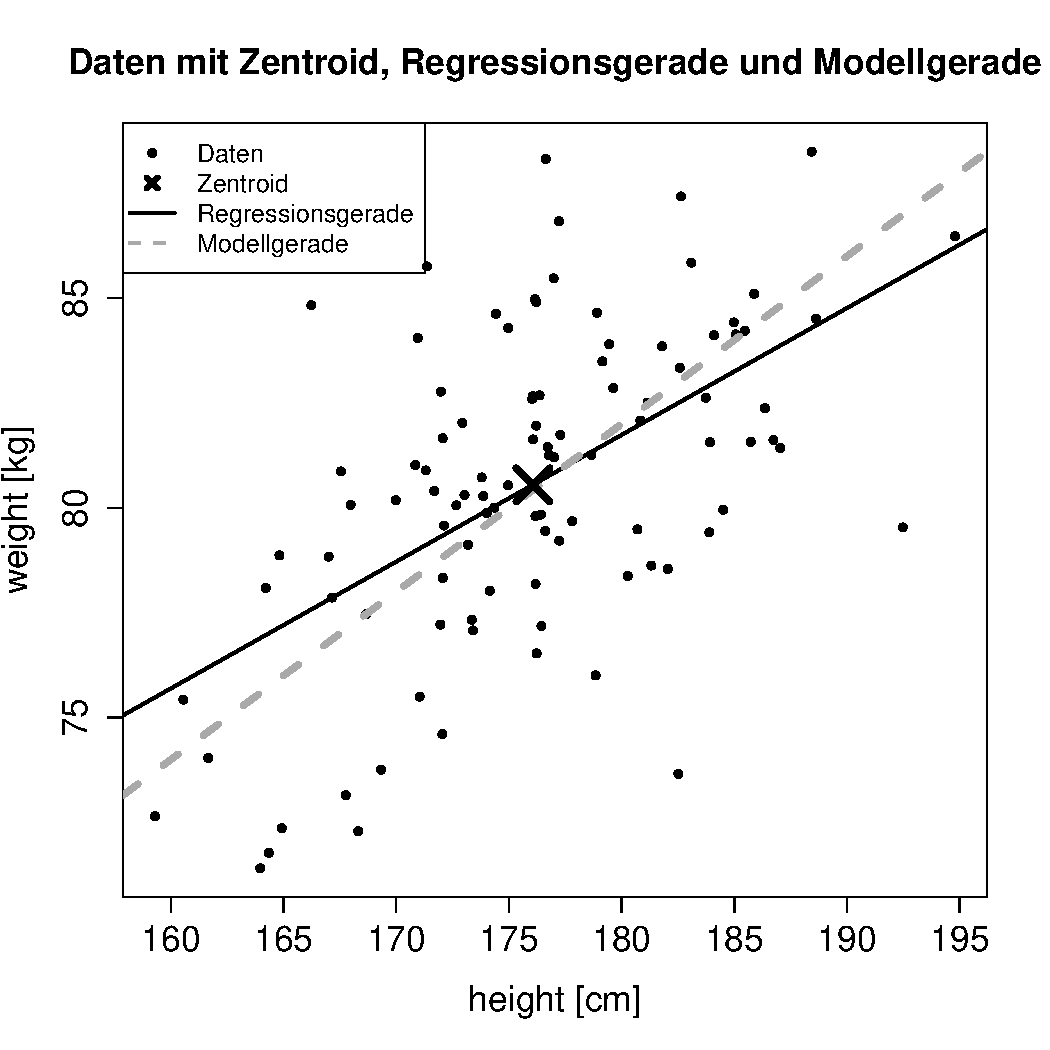
\includegraphics[width=8cm]{regrSimple}
\vspace*{-1em}
\caption{Lineare Regression: Darstellung der Daten mit Modell- und Regressionsgerade}
\label{fig:regrSimple}
\end{figure}

%%%%%%%%%%%%%%%%%%%%%%%%%%%%%%%%%%%%%%%%%%%%%%%%%%%%%%%%%%%%%%%%%%
%%%%%%%%%%%%%%%%%%%%%%%%%%%%%%%%%%%%%%%%%%%%%%%%%%%%%%%%%%%%%%%%%%
\subsection{Regressionsanalyse}
\label{sec:regrAnalysis}
%%%%%%%%%%%%%%%%%%%%%%%%%%%%%%%%%%%%%%%%%%%%%%%%%%%%%%%%%%%%%%%%%%
%%%%%%%%%%%%%%%%%%%%%%%%%%%%%%%%%%%%%%%%%%%%%%%%%%%%%%%%%%%%%%%%%%

\index{Regression!Regressionsanalyse}
Um weitere Informationen und insbesondere inferenzstatistische Kennwerte eines von \lstinline!lm()! erstellten Modells i.\,S.\ einer Regressionsanalyse zu erhalten, wird \lstinline!summary(<<lm-Modell>>)!\index[func]{summary()@\lstinline{summary()}} verwendet.\footnote{Für eine Mediationsanalyse\index{Regression!Mediation}\index{Mediationsanalyse|see{Regression}} mit dem Sobel-Test\index{Regression!Sobel-Test}\index{Sobel-Test|see{Regression}} vgl.\ \lstinline!sobel()!\index[func]{sobel()@\lstinline{sobel()}} aus dem\index[pack]{multilevel@\lstinline{multilevel}} \lstinline!multilevel! Paket \cite{Bliese2006}. Weitergehende Mediationsanalysen sind mit dem Paket \lstinline!mediation!\index[pack]{mediation@\lstinline{mediation}} \cite{Tingley2011} möglich.}
\begin{lstlisting}
> (sumRes <- summary(fit))               # gekürzte Ausgabe ...
Residuals:
    Min      1Q  Median      3Q     Max
-8.8433 -2.1565  0.3454  1.8255  7.5915

Coefficients:
             Estimate  Std. Error  t value  Pr(>|t|)
(Intercept)  27.33506     7.96062    3.434  0.000874 ***
height        0.30224     0.04518    6.690  1.39e-09 ***
---
Signif. codes:  0 '***' 0.001 '**' 0.01 '*' 0.05 '.' 0.1 ' ' 1

Residual standard error: 3.143 on 98 degrees of freedom
Multiple R-squared: 0.3135,  Adjusted R-squared: 0.3065
F-statistic:  44.76 on 1 and 98 DF,  p-value: 1.390e-09
\end{lstlisting}

Die Ausgabe enthält unter der Überschrift \lstinline!Residuals! eine Zusammenfassung der beobachtungsweisen Residuen. Diese sollten symmetrisch um 0 streuen. Ein deutlich von 0 abweichender Median sowie vom Betrag deutlich unterschiedliche Quartile (\lstinline!1Q!, \lstinline!3Q!) deuten auf eine schiefe Verteilung hin.

Unter \lstinline!Coefficients! werden die Koeffizienten (Spalte \lstinline!Estimate!), ihr Standardfehler (\lstinline!Std. Error!), $t$-Wert (\lstinline!t value!) und der zugehörige $p$-Wert für den zweiseitigen $t$-Test (\lstinline!Pr(>|t|)!) ausgegeben. Dieser Test wird mit der $\text{H}_{0}$ durchgeführt, dass das theoretische $\beta$-Gewicht gleich $0$ ist (Abschn.\ \ref{sec:multALMctr}). Die Größe des $p$-Wertes wird mit Sternchen hinter den Werten codiert, deren Bedeutung \lstinline!Signif. codes! beschreibt.\footnote{Im Folgenden wird dieser Teil der Ausgabe mit \lstinline!options(show.signif.stars=FALSE)!\index[func]{options()@\lstinline{options()}} unterdrückt.} Die Tabelle der Koeffizienten lässt sich mit \lstinline!coef()! extrahieren.
\begin{lstlisting}
# geschätzte Koeffizienten, Standardfehler, t-Werte und p-Werte
> coef(sumRes)
              Estimate Std. Error  t value     Pr(>|t|)
(Intercept) 27.3350625 7.96061681 3.433787 8.737358e-04
height       0.3022421 0.04517855 6.689947 1.390238e-09

# Streuung der Schätzungen: Wurzel aus Diagonale der Kovarianzmatrix
> (sdCoef <- sqrt(diag(vcov(fit))))
(Intercept)      height
 7.96061681  0.04517855

> (tVals <- coef(fit) / sdCoef)                  # t-Werte
(Intercept)    height
   3.433787  6.689947
\end{lstlisting}

\lstinline!Residual standard error! gibt den Standardschätzfehler als Maß für die Diskrepanz zwischen empirischen Werten des Kriteriums und der Modellvorhersage aus. Er ist gleich der Wurzel aus der mittleren Quadratsumme der Residuen als Schätzung der Fehlervarianz, also aus dem Quotienten der Quadratsumme der Residuen und ihrer Freiheitsgrade.
\begin{lstlisting}
# Freiheitsgrade der Residual-Quadratsumme, vgl. fit$df.residual
> P      <- 1                                    # Anzahl Prädiktoren
> (dfSSE <- N - (P+1))                           # Freiheitsgrade
[1] 98

> (SSE <- sum(residuals(fit)^2))                 # QS Residuen
[1] 742.2144

> deviance(fit)                                  # Kontrolle ...
> MSE <- SSE / dfSSE                             # mittlere QS Residuen
> sqrt(MSE)                                      # Standardschätzfehler
[1] 3.143246
\end{lstlisting}

\index{Determinationskoeffizient|see{Regression}}
\index{Regression!Determinationskoeffizient $R^{2}$}
Ein weiteres Maß für die Güte der Schätzung ist der Determinationskoeffizient $R^{2}$, in Modellen mit absolutem Term gleich der quadrierten Korrelation zwischen Vorhersage und Kriterium (\lstinline!Multiple R-squared!, auch multiple Korrelation\index{Korrelation!multiple Korrelation} zwischen Prädiktoren und Kriterium genannt). Das nach Wherry korrigierte $R^{2}$ (\lstinline!Adjusted R-squared!) ist eine lineare Transformation von $R^{2}$ und stimmt mit ihm überein, wenn $R^{2}$ gleich $1$ ist. Im Gegensatz zum empirischen kann das korrigierte $R^{2}$ auch negativ werden.
\begin{lstlisting}
# unkorrigiertes R^2: quadrierte Korrelation Vorhersage mit Kriterium
> Yhat <- fitted(fit)                            # Vorhersage
> (rSq <- cor(Yhat, weight)^2                    # unkorrigiertes R^2
[1] 0.3135111

> 1 - ((N-1) / (N-P-1)) * (1-rSq)                # korrigiertes R^2
[1] 0.3065061
\end{lstlisting}

%Alternativ ergibt sich das korrigierte $R^{2}$ aus der Differenz von $1$ und dem Quotienten aus der mittleren %Quadratsumme der Residuen und der mittleren Quadratsumme des Kriteriums.
%\begin{lstlisting}
%# Quadratsumme des Kriteriums -> N * unkorrigierte Varianz
%> SScrit   <- sum((weight - mean(weight))^2)
%> dfSScrit <- N-1                                 # df QS Kriterium
%> 1 - (MSE / (SScrit / dfSScrit))                 # korrigiertes R^2
%[1] 0.3065061
%\end{lstlisting}

Schließlich wird mit einem $F$-Test für das gesamte Modell die $\text{H}_{0}$ geprüft, dass (bei einer multiplen Regression, s.\ Abschn.\ \ref{sec:regrMultAn}) alle theoretischen $\beta_{j}$-Gewichte gleich $0$ sind (Abschn.\ \ref{sec:multALMmodCmp}, \ref{sec:multALMtest}). Die Einzelheiten des Tests sind der empirische Wert des $F$-Bruchs (\lstinline!F-statistic!) gefolgt von den Freiheitsgraden (\lstinline!DF!) der Vorhersage und der Residuen sowie dem $p$-Wert (\lstinline!p-value!).
\begin{lstlisting}
> MSpred <- sum((Yhat - mean(Yhat))^2) / P       # mittl. QS Vorhersage
> (Fval  <- MSpred / MSE)                        # Teststatistik F-Wert
[1] 44.75539

(pVal <- pf(Fval, P, dfSSE, lower.tail=FALSE))   # p-Wert
[1] 1.390238e-09
\end{lstlisting}

Für die geschätzten Parameter\index{Regression!Konfidenzintervall} errechnet\index[func]{confint()@\lstinline{confint()}} \lstinline!confint(<<lm-Modell>>, level=0.95)! das Konfidenzintervall mit der für das Argument \lstinline!level! angegebenen Breite.
\begin{lstlisting}
> confint(fit)
                 2.5 %     97.5 %
(Intercept) 11.5374776 43.1326475
height       0.2125868  0.3918975
\end{lstlisting}

Die Informationskriterien\index{AIC}\index{BIC} nach Akaike und Bayes (BIC) berücksichtigen einerseits die Güte der Modellpassung i.\,S.\ ihrer maximierten logarithmierten likelihood und bestrafen andererseits die Komplexität des Modells, gemessen an der Anzahl zu schätzender Parameter.\footnote{AIC und BIC besitzen einen engen Bezug zu bestimmten Methoden der Kreuzvalidierung (Abschn.\ \ref{sec:regrCV}).} Kleinere Werte stehen für eine höhere Informativität. Bei einer linearen Regression ergibt sich der AIC-Wert direkt aus der Quadratsumme der Residuen sowie der Anzahl zu schätzender Parameter: Bei $p+1$ Koeffizienten für $p$ Prädiktoren und den $y$-Achsenabschnitt sind dies $p+1+1$.\footnote{Zusätzlich zu $\beta_{0}$ und den $\beta_{j}$ ist auch die Fehlerstreuung $\sigma$ zu schätzen.} Besitzen zwei Modelle dieselbe Anpassungsgüte, erhält das Modell mit einer geringeren Anzahl von Parametern den kleineren AIC- bzw.\ BIC-Wert. Beide Werte werden durch\index[func]{extractAIC()@\lstinline{extractAIC()}} \lstinline!extractAIC(<<lm-Modell>>)! für ein Modell berechnet, wobei für BIC das Argument \lstinline!k=log(<<Stichprobengröße>>)! zu setzen ist.\footnote{Der korrigierte\index{AICc} AICc Wert für kleine Stichproben ist mit \index[func]{aictab()@\lstinline{aictab()}} \lstinline!aictab()! aus dem Paket \index[pack]{AICcmodavg@\lstinline{AICcmodavg}} \lstinline!AICcmodavg! \cite{Mazerolle2013} berechenbar.} \lstinline!AIC(<<lm-Modell>>)!\index[func]{AIC()@\lstinline{AIC()}} berechnet den AIC-Wert mit einer anders gewählten Konstante, was die für Modellvergleiche wesentliche Differenz zweier AIC-Werte aber nicht beeinflusst (Abschn.\ \ref{sec:regrCmp}). Die Ausgabe führt als erstes Element die Anzahl zu schätzender Parameter auf.
\begin{lstlisting}
> extractAIC(fit)                   # AIC-Wert
[1] 2.0000 231.0309

> extractAIC(fit, k=log(N))         # BIC-Wert
[1] 2.0000 236.2413

> N * log(SSE / N) + 2*(1+1)        # Kontrolle: AIC ...
> AIC(fit)                          # AIC-Berechnung: andere Konstante
[1] 787.1703

> N * (log(2*pi) + log(SSE / N) + 1) + 2*(1+1+1)     # Kontrolle ...
\end{lstlisting}

%%%%%%%%%%%%%%%%%%%%%%%%%%%%%%%%%%%%%%%%%%%%%%%%%%%%%%%%%%%%%%%%%%
%%%%%%%%%%%%%%%%%%%%%%%%%%%%%%%%%%%%%%%%%%%%%%%%%%%%%%%%%%%%%%%%%%
\section{Multiple lineare Regression}
\label{sec:regrMult}
%%%%%%%%%%%%%%%%%%%%%%%%%%%%%%%%%%%%%%%%%%%%%%%%%%%%%%%%%%%%%%%%%%
%%%%%%%%%%%%%%%%%%%%%%%%%%%%%%%%%%%%%%%%%%%%%%%%%%%%%%%%%%%%%%%%%%

\index{Regression!lineare}
Bei der multiplen linearen Regression dienen mehrere quantitative oder dichotome Variablen $X_{j}$ als Prädiktoren zur Vorhersage des quantitativen Kriteriums $Y$.\footnote{Für die multivariate multiple Regression mit mehreren Kriteriumsvariablen $Y_{k}$ s.\ Abschn.\ \ref{sec:multRegrMult}. Eine formalere Behandlung des allgemeinen linearen Modells findet sich in Abschn.\ \ref{sec:multALM}.} Die Vorhersagegleichung hat hier die Form $\hat{Y} = b_{0} + b_{1} X_{1} + {\dots} + b_{j} X_{j} + {\dots} + b_{p} X_{p}$, wobei die Parameter $b_{0}$ und $b_{j}$ auf Basis der empirischen Daten zu schätzen sind. Dies geschieht wie im Fall der einfachen linearen Regression mit \lstinline!lm(<<Modellformel>>)!\index[func]{lm()@\lstinline{lm()}} nach dem Kriterium der kleinsten Summe der quadrierten Abweichungen von Vorhersage und Kriterium. Die Modellformel hat nun die Form \lstinline!<<Kriterium>> ~ <<Prädiktor 1>> + ... + <<Prädiktor p>>!, d.\,h.\ alle $p$ Prädiktoren $X_{j}$ werden mit \lstinline!+! verbunden auf die Rechte Seite der \lstinline!~! geschrieben.

%%%%%%%%%%%%%%%%%%%%%%%%%%%%%%%%%%%%%%%%%%%%%%%%%%%%%%%%%%%%%%%%%%
%%%%%%%%%%%%%%%%%%%%%%%%%%%%%%%%%%%%%%%%%%%%%%%%%%%%%%%%%%%%%%%%%%
\subsection{Deskriptive Modellanpassung und Regressionsanalyse}
\label{sec:regrMultAn}
%%%%%%%%%%%%%%%%%%%%%%%%%%%%%%%%%%%%%%%%%%%%%%%%%%%%%%%%%%%%%%%%%%
%%%%%%%%%%%%%%%%%%%%%%%%%%%%%%%%%%%%%%%%%%%%%%%%%%%%%%%%%%%%%%%%%%

Als Beispiel soll nun \lstinline!weight! wie bisher aus der Körpergröße \lstinline!height! vorhergesagt werden, aber auch mit Hilfe des Alters \lstinline!age! und später ebenfalls mit der Anzahl der Minuten, die pro Woche Sport getrieben wird (\lstinline!sport!). Der Simulation der Daten wird die Gültigkeit eines entsprechenden linearen Modells mit zufälligen Fehlern zugrundegelegt.
\begin{lstlisting}
> N      <- 100                                  # Anzahl Personen
> height <- rnorm(N, mean=175, sd=7)             # Prädiktor 1
> age    <- rnorm(N, mean=30, sd=8)              # Prädiktor 2
> sport  <- abs(rnorm(N, mean=60, sd=30))        # Prädiktor 3

# Simulation des Kriteriums im Modell der multiplen linearen Regression
> weight <- 0.5*height - 0.3*age - 0.4*sport + 10 + rnorm(N, 0, 3)
> (fitHA <- lm(weight ~ height + age))           # gekürzte Ausgabe ...
Coefficients:
(Intercept)  height      age
   -72.5404  0.8602  -0.4429
\end{lstlisting}

Die Schätzungen $b_{0}$ und $b_{j}$ der theoretischen Parameter $\beta_{0}$ und $\beta_{j}$ werden in der Ausgabe unter der Überschrift \lstinline!Coefficients! genannt, wobei $b_{0}$ in der Spalte \lstinline!(Intercept)! und die $b_{j}$-Gewichte unter dem Namen des zugehörigen Prädiktors stehen. Auch hier müssen die Variablen in der Modellformel $z$-standardisiert werden, um die standardisierten $b_{j}^{z}$-Gewichte zu berechnen (s.\ Abschn.\ \ref{sec:regrSimpleDescr}, Fußnote \ref{ftn:scaleNA} für das Vorgehen bei fehlenden Werten). Wie im Fall einer einfachen linearen Regression werden die Parameter mit \lstinline!summary(<<lm-Modell>>)! auf Signifikanz getestet (Abschn.\ \ref{sec:regrAnalysis}).
\begin{lstlisting}
# für standardisierte b-Gewichte
> lm(scale(weight) ~ scale(height) + scale(age)) # ...
> summary(fitHA)                               # Regressionsanalyse ...
\end{lstlisting}

Ist $\bm{X}$ die mit \lstinline!model.matrix(<<lm-Modell>>)! erzeugte Designmatrix i.\,S.\ des allgemeinen linearen Modells und $\bm{y}$ der Vektor der Kriteriumswerte, lassen sich die Schätzungen $b_{0}$ und $b_{j}$ als $\bm{X}^{+} \bm{y}$ berechnen (mit der\index{Matrix!Pseudoinverse} Pseudoinversen $\bm{X}^{+}$ von $\bm{X}$).\footnote{Es sei vorausgesetzt, dass $\bm{X}$ vollen Spaltenrang hat, also keine linearen Abhängigkeiten zwischen den Prädiktoren vorliegen. Dann gilt $\bm{X}^{+} = (\bm{X}^{\top} \bm{X})^{-1} \bm{X}^{\top}$. Der hier gewählte Rechenweg ist numerisch nicht stabil und weicht von in R-Funktionen implementierten Rechnungen ab \cite{Bates2004}.} Der Vektor der vorhergesagten Werte berechnet sich als $\hat{\bm{y}} = \bm{H} \bm{y}$ (mit der\index{Regression!Hat-Matrix} \emph{Hat-Matrix} $\bm{H} = \bm{X} \bm{X}^{+}$, s.\ Abschn.\ \ref{sec:matOrthProj}, \ref{sec:multALMregr}, \ref{sec:multALMpred}).
\begin{lstlisting}
# Koeffizienten aus Produkt der Pseudoinversen X+ mit Kriterium
> X     <- model.matrix(fitHA)                    # Designmatrix
> Xplus <- solve(t(X) %*% X) %*% t(X)             # Pseudoinverse X+
> (b    <- Xplus %*% weight)                      # Parameterschätzung
(Intercept) -72.5404499
height        0.8602345
age          -0.4428933

# Vorhersage aus Produkt der Hat-Matrix mit Kriterium
> H    <- X %*% Xplus                             # Hat-Matrix
> Yhat <- H %*% weight                            # Vorhersage
> all.equal(fitted(fitHA), c(Yhat), check.attributes=FALSE)
[1] TRUE

# bz-Gewichte bei standardisierten Variablen
> S <- cov(cbind(height, age))        # Kovarianzmatrix Prädiktoren
> (1/sd(weight)) * diag(sqrt(diag(S))) %*% b[-1]  # Kontrolle ...
\end{lstlisting}

\index{Regression!grafische Darstellung}
Die grafische Veranschaulichung mit\index[func]{scatter3d()@\lstinline{scatter3d()}} \lstinline!scatter3d()! aus dem Paket\index[pack]{car@\lstinline{car}} \lstinline!car! zeigt die simulierten Daten zusammen mit der Vorhersageebene sowie die Residuen als vertikale Abstände zwischen ihr und den Daten (Abb.\ \ref{fig:regrMult}). Als Argument ist dieselbe Modellformel wie für \lstinline!lm()! zu verwenden. Weitere Argumente kontrollieren das Aussehen der Diagrammelemente. Die Beobachterperspektive dieser Grafik lässt sich interaktiv durch Klicken und Ziehen mit der Maus ändern (Abschn.\ \ref{sec:3dGrid}).
\begin{lstlisting}
> library(car)                                    # für scatter3d()
> scatter3d(weight ~ height + age, fill=FALSE)
\end{lstlisting}

\begin{figure}[ht]
\centering
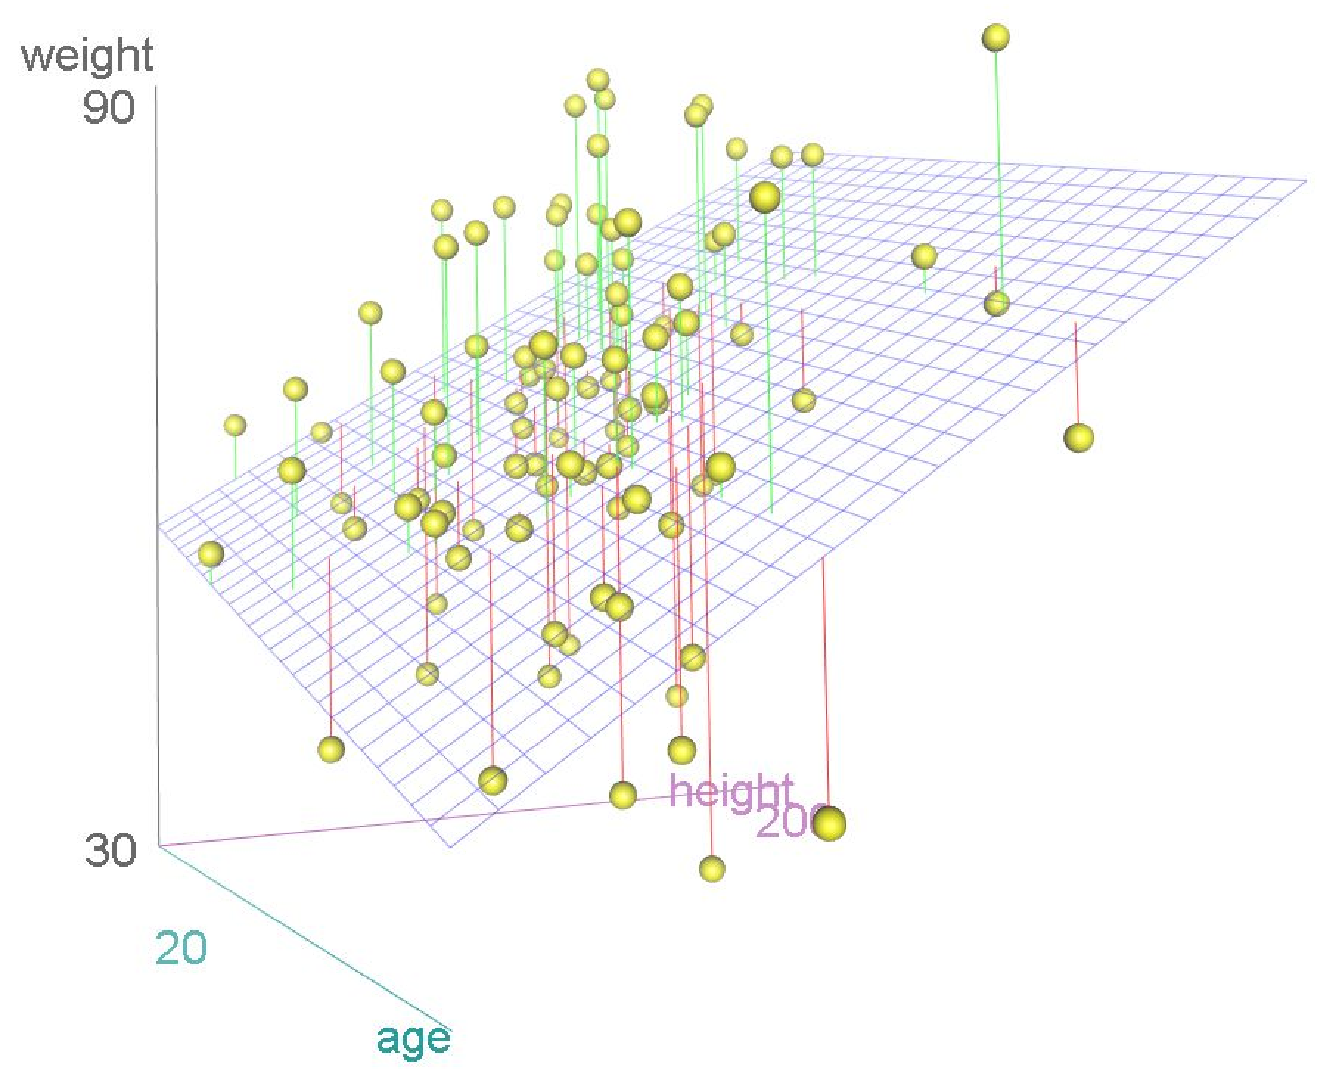
\includegraphics[width=8cm]{regrMult}
\vspace*{-1em}
\caption{Daten, Vorhersageebene und Residuen einer multiplen linearen Regression}
\label{fig:regrMult}
\end{figure}

%%%%%%%%%%%%%%%%%%%%%%%%%%%%%%%%%%%%%%%%%%%%%%%%%%%%%%%%%%%%%%%%%%
%%%%%%%%%%%%%%%%%%%%%%%%%%%%%%%%%%%%%%%%%%%%%%%%%%%%%%%%%%%%%%%%%%
\subsection{Modell verändern}
\label{sec:regrUpdate}
%%%%%%%%%%%%%%%%%%%%%%%%%%%%%%%%%%%%%%%%%%%%%%%%%%%%%%%%%%%%%%%%%%
%%%%%%%%%%%%%%%%%%%%%%%%%%%%%%%%%%%%%%%%%%%%%%%%%%%%%%%%%%%%%%%%%%

\index{Regression!Modell verändern}
\index[func]{update()@\lstinline{update()}}
Möchte man ein bereits berechnetes Modell nachträglich verändern, ihm etwa einen weiteren Prädiktor hinzufügen, kann dies mit \lstinline!update()! geschehen. Bei sehr umfassenden Modellen kann dies numerisch effizienter sein, als ein Modell vollständig neu berechnen zu lassen.
\begin{lstlisting}
update(<<lm-Modell>>, . ~ . + <<weiterer Prädiktor>>)
\end{lstlisting}

Als erstes Argument wird das zu erweiternde Modell eingetragen. Die folgende Modellformel \lstinline!. ~ .! signalisiert, dass alle bisherigen Prädiktoren beizubehalten sind. Jeder weitere Prädiktor wird dann mit einem \lstinline!+! angefügt. Das Ergebnis von \lstinline!update()! ist das aktualisierte Modell.
\begin{lstlisting}
# füge sport als zusätzlichen Prädiktor hinzu
> (fitHAS <- update(fitHA, . ~ . + sport))     # gekürzte Ausgabe ...
Coefficients:
(Intercept)  height      age    sport
     8.1012  0.5149  -0.2866  -0.4160
\end{lstlisting}

Auf die gleiche Weise wie Prädiktoren hinzugefügt werden können, lassen sie sich auch entfernen, wobei statt des \lstinline!+! ein \lstinline!-! zu verwenden ist.
\begin{lstlisting}
# entferne Prädiktor height
> (fitAS <- update(fitHAS, . ~ . - height))     # gekürzte Ausgabe ...
Coefficients:
(Intercept)      age    sport
    98.5145  -0.2459  -0.4452

> (fitH <- update(fitHA,  . ~ . - age))         # entferne age ...
\end{lstlisting}

%%%%%%%%%%%%%%%%%%%%%%%%%%%%%%%%%%%%%%%%%%%%%%%%%%%%%%%%%%%%%%%%%%
%%%%%%%%%%%%%%%%%%%%%%%%%%%%%%%%%%%%%%%%%%%%%%%%%%%%%%%%%%%%%%%%%%
\subsection{Modelle vergleichen und auswählen}
\label{sec:regrCmp}
%%%%%%%%%%%%%%%%%%%%%%%%%%%%%%%%%%%%%%%%%%%%%%%%%%%%%%%%%%%%%%%%%%
%%%%%%%%%%%%%%%%%%%%%%%%%%%%%%%%%%%%%%%%%%%%%%%%%%%%%%%%%%%%%%%%%%

\index{Regression!Modellvergleich}
\index{Regression!hierarchische}
Existieren bei einer multiplen Regression viele potentielle Prädiktoren, stellt sich die Frage, welche letztlich im Modell berücksichtigt werden sollten. In einem hierarchischen Vorgehen lässt sich dafür testen, inwieweit die Hinzunahme von Prädiktoren zu einer bedeutsamen Verbesserung der Modellpassung führt. Dies ist in Form von $F$-Tests über Modellvergleiche möglich, die die Veränderung der Residualvarianz in Abhängigkeit vom verwendeten Prädiktorensatz testen. Dabei lassen sich sinnvoll nur \emph{nested} Modelle mit demselben Kriterium vergleichen, bei denen der Prädiktorensatz eines eingeschränkten Modells vollständig im Prädiktorensatz des umfassenderen Modells enthalten ist, das zusätzlich noch weitere Prädiktoren berücksichtigt (Abschn.\ \ref{sec:multALMmodCmp}).

Um verschiedene Regressionsmodelle miteinander hinsichtlich der Quadratsumme der Residuen sowie Akaikes Informationskriterium AIC vergleichen zu können, lassen sich folgende Funktionen verwenden:
\index[func]{step()@\lstinline{step()}}
\index[func]{add1()@\lstinline{add1()}}
\index[func]{drop1()@\lstinline{drop1()}}
\begin{lstlisting}
 step(object=<<lm-Modell>>, scope=~ . + <<Prädiktoren>>, direction="both)
 add1(object=<<lm-Modell>>, scope=~ . + <<Prädiktoren>>, test="none")
drop1(object=<<lm-Modell>>, scope=~ . - <<Prädiktoren>>, test="none")
\end{lstlisting}

\lstinline!step()! berechnet im \emph{Stepwise}-Verfahren\index{Regression!Stepwise-Verfahren} die Auswirkung einer schrittweisen Modellveränderung durch Hinzunahme oder Weglassen eines Prädiktors auf den AIC-Wert als Vergleichskriterium für die Güte der Modellpassung. Als Ergebnis wird ein Modell zurückgegeben, das durch diese Schritte nicht substantiell verbessert werden kann.\footnote{Das Paket \lstinline!leaps!\index[pack]{leaps@\lstinline{leaps}} \cite{Lumley2009} ermöglicht die automatisierte Auswahl aller Teilmengen von Prädiktoren. Beide Verfahren sind mit vielen inhaltlichen Problemen verbunden, für eine Diskussion und verschiedene Strategien zur Auswahl von Prädiktoren vgl.\ \citeA{Miller2002}. Für penalisierte Regressionsverfahren, die auch eine Auswahl von Prädiktoren vornehmen, s.\ Abschn.\ \ref{sec:lmRob}.}

Dazu prüft \lstinline!step()! sequentiell Teilmengen von denjenigen Prädiktoren der unter \lstinline!object! angegebenen Regression, die in \lstinline!scope! als Modellformel definiert werden. Diese Modellformel beginnt mit einer \lstinline!~! und enthält danach alle Prädiktoren aus \lstinline!object! (Voreinstellung \lstinline!~ .!) sowie ggf.\ weitere mit \lstinline!+! hinzuzufügende. Mit \lstinline!step="backward"! beginnt die Exploration der Modelle beim umfassendsten Modell und entfernt dann Prädiktoren (Rückwärts-Elimination), analog mit \lstinline!step="forward"! beim einfachsten Modell und fügt Prädiktoren hinzu (Vorwärts-Selektion). In der Voreinstellung \lstinline!direction="both"! können von Schritt zu Schritt Prädiktoren sowohl hinzugefügt als auch entfernt werden.
\begin{lstlisting}
# Vorwärts-Selektion
> step(fitH, scope="~ height + age + sport", direction="forward")
Start:  AIC=501.38
weight ~ height
        Df Sum of Sq     RSS    AIC
+ sport  1   12962.8  1495.1 276.48
+ age    1    1246.3 13211.6 494.37
<none>               14457.9 501.38

Step:  AIC=276.48
weight ~ height + sport
       Df Sum of Sq     RSS    AIC
+ age   1     515.5  979.64 236.20
<none>              1495.14 276.48

Step:  AIC=236.2
weight ~ height + sport + age
Coefficients:
(Intercept)       height        sport          age  
     8.1012       0.5149      -0.4160      -0.2866 
\end{lstlisting}

\lstinline!add1()! berechnet separat den Effekt der Hinzunahme jeweils eines unter \lstinline!scope! genannten Prädiktors zu einer unter \lstinline!object! angegebenen Regression. Die Änderung in der Quadratsumme der Residuen bei jedem Schritt kann inferenzstatistisch geprüft werden, indem das Argument \lstinline!test="F"! gesetzt wird. Das einfachste Modell, in dem kein Prädiktor berücksichtigt wird, lautet \lstinline!<<Kriterium>> ~ 1! und sorgt dafür, dass für jeden Wert der konstante Mittelwert des Kriteriums vorhergesagt wird.
\begin{lstlisting}
# Vergleich: nur height als Prädiktor, sowie auch age bzw. sport
> add1(fitH, . ~ . + age + sport, test="F")
Single term additions
Model:
weight ~ height
        Df  Sum of Sq      RSS     AIC  F value     Pr(>F)
<none>                 14457.9  501.38
age      1     1246.3  13211.6  494.37     9.15   0.003183 **
sport    1    12962.8   1495.1  276.48   840.98  < 2.2e-16 ***
\end{lstlisting}

In der Zeile \lstinline!<none>! der Ausgabe finden sich die Kennwerte des eingeschränkten \lstinline!object! Modells. Die folgenden Zeilen nennen die Kennwerte der umfassenderen Modelle, bei denen zusätzlich jeweils einer der unter \lstinline!scope! genannten Prädiktoren berücksichtigt wird. Die Spalte \lstinline!Sum of Sq! führt die\index{Quadratsummen-Typen|see{Varianzanalyse}}\index{Varianzanalyse!Quadratsummen-Typen} sequentielle Quadratsumme vom Typ I des zusätzlichen Prädiktors beim Wechsel hin zu einem solchen Modell auf. Sie ist gleich der Differenz der in der Spalte \lstinline!RSS! genannten Quadratsummen der Residuen (\emph{residual sum of squares}) und damit ein Maß für die Reduktion an Fehlervarianz beim Modellwechsel. Die inferenzstatistischen Kennwerte finden sich in den Spalten \lstinline!Df! für die Differenz der Fehler-Freiheitsgrade vom eingeschränkten und umfassenderen Modell, \lstinline!F value! für den $F$-Wert und \lstinline!Pr(>F)! für den $p$-Wert. Auf ähnliche Weise kann mit \lstinline!drop1()! die Quadratsumme vom Typ III eines Vorhersageterms als Effekt des Weglassens jeweils eines Prädiktors berechnet werden (Abschn.\ \ref{sec:ssTypes}).

Der $F$-Wert ergibt sich als Quotient der angegebenen Quadratsumme geteilt durch die Differenz der Fehler-Freiheitsgrade und der Residual-Quadratsumme des umfassenderen Modells geteilt durch ihre Freiheitsgrade (Abschn.\ \ref{sec:multALMtest}). Die Fehler-Freiheitsgrade eines Modells berechnen sich als Differenz zwischen der Stichprobengröße und der Anzahl zu schätzender Parameter. Hier sind dies im eingeschränkten Modell mit einem Regressionsgewicht und dem absoluten Term zwei, in jedem Modell mit einem zusätzlichen Prädiktor entsprechend drei.
\begin{lstlisting}
# RSS Zeile <none>: Prädiktor height
> (rssH <- sum(residuals(lm(weight ~ height))^2))
[1] 14457.9

# RSS Zeile age: Prädiktoren height und age
> (rssHA <- sum(residuals(lm(weight ~ height + age))^2))
[1] 13211.64

# RSS Zeile sport: Prädiktoren height und sport
> (rssHS <- sum(residuals(lm(weight ~ height + sport))^2))
[1] 1495.140

# Fehler-Freiheitsgrade der drei Modelle
> dfEH  <- N - (1+1)                # eingeschränktes Modell
> dfEHA <- dfEHS <- N - (2+1)       # beide umfassenderen Modelle

# mittlere partielle Effekt-QS für Hinzunahme von age
> MSha <- (rssH - rssHA) / (dfEH - dfEHA)

# mittlere Residual-QS umfassenderes Modell: Prädiktoren height und age
> MSEha <- rssHA / dfEHA

# F-Wert für Effekt der Hinzunahme von age
> (Fha <- MSha / MSEha)
[1] 9.150025

# analog für Hinzunahme von sport
> MShs  <- (rssH - rssHS) / (dfEH - dfEHS)
> MSEhs <- rssHS / dfEHS
> (Fhs  <- MShs / MSEhs)
[1] 840.9835
\end{lstlisting}

Die Spalte \lstinline!AIC! listet den Wert von Akaikes Informationskriterium für beide Modelle auf.

Um nested Modelle gegeneinander zu testen, die sich um mehr als einen Prädiktor unterscheiden, können mit \lstinline!lm()! erstellte Regressionen an die\index[func]{anova()@\lstinline{anova()}} \lstinline!anova()! Funktion übergeben werden, die sich auch für Varianzanalysen eignet (Abschn.\ \ref{sec:anova}). Die Modelle müssen sich auf dieselben Beobachtungen beziehen -- bei fehlenden Werten ist sicherzustellen, dass in beide Modelle dieselben Beobachtungen einfließen.
\begin{lstlisting}
anova(<<eingeschränktes lm-Modell>>, <<umfassenderes lm-Modell>>)
\end{lstlisting}

Im Beispiel soll das Kriterium \lstinline!weight! entweder nur durch \lstinline!height!, oder aber durch alle drei Prädiktoren vorhergesagt werden.
\begin{lstlisting}
> anova(fitH, fitHAS)       # F-Test für Hinzunahme von age und sport
Analysis of Variance Table
Model 1: weight ~ height
Model 2: weight ~ height + age + sport
  Res.Df      RSS  Df  Sum of Sq      F     Pr(>F)
1     98  14457.9
2     96    979.6   2      13478  660.4  < 2.2e-16 ***
\end{lstlisting}

In der Ausgabe wird in der Spalte \lstinline!RSS! die Residual-Quadratsumme für jedes Modell aufgeführt, die zugehörigen Freiheitsgrade in der Spalte \lstinline!Res.Df!. In der Spalte \lstinline!Df! steht deren Differenz, um wie viele Parameter sich die Modelle also unterscheiden. Die Reduktion der Residual-Quadratsumme beim Wechsel zum umfassenderen Modell findet sich in der Spalte \lstinline!Sum of Sq!, daneben der zugehörige $F$-Wert (\lstinline!F!) und $p$-Wert (\lstinline!Pr(>F)!).

%%%%%%%%%%%%%%%%%%%%%%%%%%%%%%%%%%%%%%%%%%%%%%%%%%%%%%%%%%%%%%%%%%
%%%%%%%%%%%%%%%%%%%%%%%%%%%%%%%%%%%%%%%%%%%%%%%%%%%%%%%%%%%%%%%%%%
\subsection{Moderierte Regression}
\label{sec:regrMod}
%%%%%%%%%%%%%%%%%%%%%%%%%%%%%%%%%%%%%%%%%%%%%%%%%%%%%%%%%%%%%%%%%%
%%%%%%%%%%%%%%%%%%%%%%%%%%%%%%%%%%%%%%%%%%%%%%%%%%%%%%%%%%%%%%%%%%

\index{Regression!Moderation}
\index{Regression!Interaktion}
Bei der multiplen Regression kann die Hypothese bestehen, dass die theoretischen Regressionsparameter eines Prädiktors von der Ausprägung eines anderen Prädiktors abhängen \cite{Aiken1991}. Im Rahmen eines einfachen kausalen Einflussmodells mit einem Prädiktor (UV), einem Kriterium (AV) und einer Drittvariable ließe sich etwa vermuten, dass der Einfluss der UV auf die AV davon abhängt, wie die Drittvariable ausgeprägt ist.\footnote{Für Hinweise zur Analyse komplexerer Kausalmodelle s.\ Abschn.\ \ref{sec:multFA}, Fußnote \ref{ftn:structEqMod}.} Bei quantitativen Variablen spricht man dann von einer \emph{Moderation}, während man im Rahmen einer Varianzanalyse mit mehreren kategorialen UVn den Begriff der \emph{Interaktion} verwendet (Abschn.\ \ref{sec:CRFpq}). Die Vorhersagegleichung der Regression mit zwei Prädiktoren erweitert sich durch den Interaktionsterm zu $\hat{Y} = b_{0} + b_{1} X_{1} + b_{2} X_{2} + b_{3} (X_{1} X_{2})$. Es wird also einfach ein weiterer Vorhersageterm hinzugefügt, der gleich dem Produkt beider Prädiktoren ist. Im Aufruf von \lstinline!lm()! geschieht dies durch Aufnahme des Terms \lstinline!X1:X2! in die Modellformel.

Im umgeformten Modell $\hat{Y} = (b_{0} + b_{2} X_{2}) + (b_{1} + b_{3} X_{2}) X_{1}$ wird ersichtlich, dass es sich wie jenes der einfachen linearen Regression des Prädiktors $X_{1}$ schreiben lässt, wobei $y$-Achsenabschnitt und Steigungsparameter nun lineare Funktionen des als Moderator betrachteten Prädiktors $X_{2}$ sind. Der Term $b_{0s} = b_{0} + b_{2} X_{2}$ wird als \emph{simple intercept}, $b_{1s} = b_{1} + b_{3} X_{2}$ als \emph{simple slope} bezeichnet. Für einen festen Wert des Moderators $X_{2}$ ergeben sich für $b_{0s}$ und $b_{1s}$ konkrete Werte, die dann \emph{bedingte} Koeffizienten heißen. Um einen Eindruck von der Bandbreite der Parameterschätzungen zu gewinnen, bieten sich für die Wahl fester Werte von $X_{2}$ dessen Mittelwert sowie die Werte $\pm$ eine Standardabweichung um den Mittelwert an. Eine andere Möglichkeit sind der Median sowie das erste und dritte Quartil von $X_{2}$.

\index[func]{plotSlopes()@\lstinline{plotSlopes()}}
\lstinline!plotSlopes()! aus dem Paket \lstinline!rockchalk!\index[pack]{rockchalk@\lstinline{rockchalk}} \cite{Johnson2013} berechnet die bedingten Koeffizienten für vorgegebene Werte des Moderators -- auch für Modelle mit einem Moderator, aber noch weiteren Prädiktoren, die nicht Teil einer Interaktion sind.
\begin{lstlisting}
plotSlopes(<<lm-Modell>>, plotx="<<Prädiktor>>", modx="<<Moderator>>",
           modxVals="<<Moderator-Werte>>")
\end{lstlisting}

Als erstes Argument ist ein mit \lstinline!lm()! erstelltes Regressionsmodell zu übergeben. \lstinline!plotx! erwartet den Namen von $X_{1}$, also der Variable, die Teil der Interaktion mit dem Moderator ist. Im ausgegebenen Streudiagramm definiert sie die $x$-Achse. Für \lstinline!modx! ist $X_{2}$ als Moderatorvariable zu nennen.\footnote{In Kovarianzanalysen (Abschn.\ \ref{sec:ancova}) kann \lstinline!modx! auch ein Faktor sein.} Für welche Werte des Moderators die bedingten Koeffizienten berechnet werden sollen, kontrolliert \lstinline!modxVals!: Auf \lstinline!"std.dev"! gesetzt sind dies der Mittelwert $\pm$ eine Standardabweichung, mit \lstinline!"quantile"! der Median sowie das erste und dritte Quartil. Das Ergebnis ist ein Streudiagramm von $X_{1}$ und $Y$, in das die zu $b_{0s}$ und $b_{1s}$ gehörenden bedingten Regressionsgeraden eingezeichnet sind (Abb.\ \ref{fig:regrModeration}). Moderator sei hier das Alter bei der Regression des Körpergewichts auf die Körpergröße.
\begin{lstlisting}
# Modell mit zentrierten Prädiktoren und Interaktionsterm
> heightC <- c(scale(height, center=TRUE, scale=FALSE))
> ageC    <- c(scale(age,    center=TRUE, scale=FALSE))
> fitHAi  <- lm(weight ~ heightC + ageC + heightC:ageC)
> coef(summary(fitHAi))
              Estimate  Std. Error  t value  Pr(>|t|)
(Intercept)   63.95331     1.17188   54.573   < 2e-16 ***
heightC        0.85591     0.16413    5.215  1.06e-06 ***
ageC          -0.44947     0.14696   -3.058   0.00288 **
heightC:ageC   0.01509     0.01945    0.776   0.43986

# Diagramm mit simple slopes für drei Werte des Moderators
> library(rockchalk)              # für plotSlopes(), testSlopes()
> ps <- plotSlopes(fitHAi, plotx="heightC", modx="ageC",
+                  modxVals="std.dev")
\end{lstlisting}

\begin{figure}[ht]
\centering
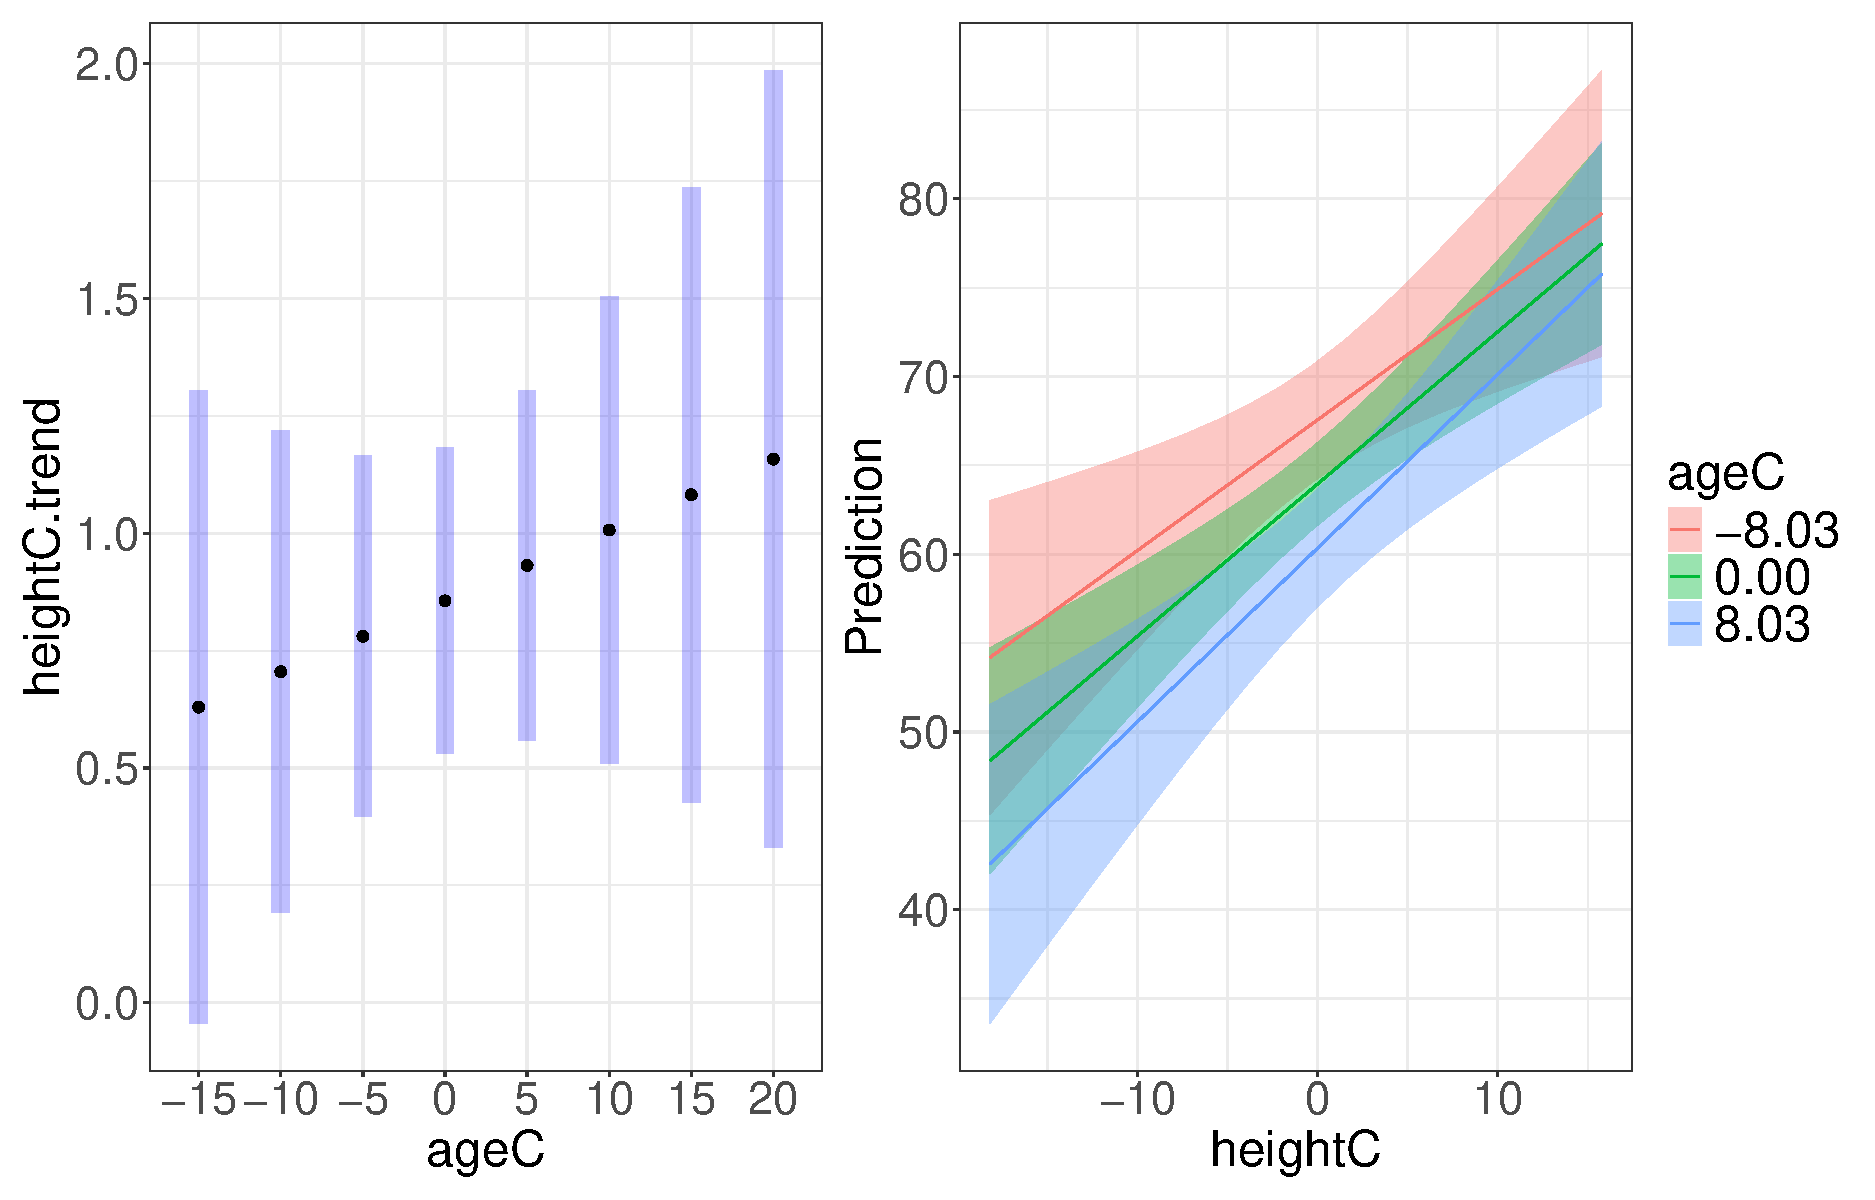
\includegraphics[width=12.5cm]{regrModeration}
\vspace*{-0.5em}
\caption{Simple slopes in der Regression mit Moderator}
\label{fig:regrModeration}
\end{figure}

\index[func]{testSlopes()@\lstinline{testSlopes()}}
Als weiteres Ergebnis liefert \lstinline!plotSlopes()! ein Objekt, das an \lstinline!testSlopes()! übergeben werden kann, um Standardabweichungen, $t$- und $p$-Werte für die Tests der bedingten Koeffizienten zu berechnen. In der von \lstinline!testSlopes()! ausgegebenen Liste stehen diese Ergebnisse in der Komponente \lstinline!hypotests!.
\begin{lstlisting}
> (ts <- testSlopes(ps))
Values of ageC INSIDE this interval:
       lo        hi
-14.08742  35.21252
cause the slope of (b1+b2*ageC)heightC to be statistically significant

$hypotests
       "ageC"     slope Std. Error  t value     Pr(>|t|)
(m-sd)  -8.03 0.7347739  0.2303663 3.189589 1.924802e-03
(m)      0.00 0.8559139  0.1641263 5.214971 1.055984e-06
(m+sd)   8.03 0.9770540  0.2226857 4.387592 2.941003e-05

...                                   # gekürzte Ausgabe
\end{lstlisting}

Die Ausgabe nennt zunächst das Johnson-Neyman Intervall als Wertebereich des Moderators, für den der Test der bedingten Steigung signifikant ist. In den Zeilen der Komponente \lstinline!hypotests! stehen die Kennwerte der bedingten Steigungen, die sich für den Mittelwert von $X_{2}$ (\lstinline!(m)!) und $\pm$ eine Standardabweichung von $X_{2}$ ergeben (\lstinline!(m-sd)! bzw.\ \lstinline!(m+sd)!). In der Spalte \lstinline!slope! findet sich die bedingte Steigung, dahinter die Standardabweichung ihrer Schätzung (\lstinline!Std. Error!) sowie der $t$-Wert (\lstinline!t value!) und der zugehörige zweiseitige $p$-Wert (\lstinline!Pr(>|t|)!).

Darüber hinaus lässt sich die von \lstinline!testSlopes()! erzeugte Liste an \lstinline!plot()! übergeben, um ein Diagramm zu erstellen, das den Konfidenzbereich um die bedingten Steigungen für den beobachteten Bereich der Werte des Moderators visualisiert (Abb.\ \ref{fig:regrModeration}).
\begin{lstlisting}
> plot(ts)      # Diagramm für Konfidenzbereich um bedingte Steigung

# manuelle Kontrolle
> coeffs <- coef(fitHAi)              # extrahiere Koeffizienten
> b0 <- coeffs[1]
> b1 <- coeffs[2]
> b2 <- coeffs[3]
> b3 <- coeffs[4]

# bedingte y-Achsenabschnitte
> b0 + b2*(mean(ageC) - sd(ageC))     # für M - 1sd ...
> b0 + b2* mean(ageC)                 # für M ...
> b0 + b2*(mean(ageC) + sd(ageC))     # für M + 1sd ...

# bedingte Steigungen
> b1 + b3*(mean(ageC) - sd(ageC))     # für M - 1sd ...
> b1 + b3* mean(ageC)                 # für M ...
> b1 + b3*(mean(ageC) + sd(ageC))     # für M + 1sd ...
\end{lstlisting}

%%%%%%%%%%%%%%%%%%%%%%%%%%%%%%%%%%%%%%%%%%%%%%%%%%%%%%%%%%%%%%%%%%
%%%%%%%%%%%%%%%%%%%%%%%%%%%%%%%%%%%%%%%%%%%%%%%%%%%%%%%%%%%%%%%%%%
\section{Regressionsmodelle auf andere Daten anwenden}
\label{sec:predict}
%%%%%%%%%%%%%%%%%%%%%%%%%%%%%%%%%%%%%%%%%%%%%%%%%%%%%%%%%%%%%%%%%%
%%%%%%%%%%%%%%%%%%%%%%%%%%%%%%%%%%%%%%%%%%%%%%%%%%%%%%%%%%%%%%%%%%

\index{Regression!Konfidenzintervall}
\index{Regression!Toleranzintervall}
\index[func]{predict()@\lstinline{predict()}}
\lstinline!predict()! wendet ein von \lstinline!lm()! angepasstes Regressionsmodell auf neue Daten an, um für sie die Vorhersage $\hat{Y}$ zu berechnen (vgl.\ \lstinline!?predict.lm!).
\begin{lstlisting}
predict(object=<<lm-Modell>>, newdata=<<Datensatz>>, se.fit=FALSE,
        interval=NULL, level=<<Breite Konfidenzintervall>>)
\end{lstlisting}

Als erstes Argument ist ein von \lstinline!lm()! erzeugtes Objekt zu übergeben. Werden alle weiteren Argumente weggelassen, liefert die Funktion die Vorhersage für die ursprünglichen Prädiktorwerte zurück, also \lstinline!fitted(<<lm-Modell>>)!. Wird unter \lstinline!newdata! ein Datensatz übergeben, der Variablen mit denselben Namen wie jene der ursprünglichen Prädiktoren enthält, so wird $\hat{Y}$ für die Werte dieser neuen Variablen berechnet.\footnote{Handelt es sich etwa im Rahmen einer Kovarianzanalyse (Abschn.\ \ref{sec:ancova}) um einen kategorialen Prädiktor -- ein Objekt der Klasse \lstinline!factor!, so muss die zugehörige Variable in \lstinline!newdata! dieselben Stufen in derselben Reihenfolge beinhalten wie die Variable des ursprünglichen Modells -- selbst wenn nicht alle Faktorstufen tatsächlich als Ausprägung vorkommen.} Wenn die Modellformel Transformationen von Variablen -- etwa mit \lstinline!I()! (Abschn.\ \ref{sec:formula}) oder \lstinline!poly()! (Abschn.\ \ref{sec:lmNonlin}) -- enthält, werden diese von \lstinline!predict()! automatisch aus den Variablen des Datensatzes gebildet. Sollen die Standardabweichungen für $\hat{Y}$ ermittelt werden, ist \lstinline!se.fit=TRUE! zu setzen.

Mit dem Argument \lstinline!interval="confidence"! berechnet \lstinline!predict()! zusätzlich für jeden Wert der Prädiktorvariablen die Grenzen des punktweisen Konfidenzintervalls für den bedingten Erwartungswert von $Y$, dessen Breite mit \lstinline!level! kontrolliert wird. Mit \lstinline!interval="prediction"! erhält man die Grenzen des Toleranzintervalls für die Vorhersage neuer Beobachtungen von $Y$. Das Toleranzintervall spiegelt einerseits die Unsicherheit der Parameterschätzer, andererseits auch die geschätzte Streuung $\hat{\sigma}$ von $Y$ um den bedingten Erwartungswert (Standardschätzfehler) wider. Die Ausgabe erfolgt in Form einer Matrix, deren erste Spalte (\lstinline!fit!) die Vorhersage ist, während die beiden weiteren Spalten untere (\lstinline!lwr!) und obere Grenzen (\lstinline!upr!) des Vertrauensbereichs nennen.

Im Beispiel des Modells mit nur dem Prädiktor \lstinline!height! wird für den Aufruf von \lstinline!predict()! zunächst ein Datensatz mit einer passend benannten Variable erzeugt.
\begin{lstlisting}
> newHeight <- c(177, 150, 192, 189, 181)         # neue Daten
> newDf     <- data.frame(height=newHeight)       # Datensatz
> predict(fitH, newDf, interval="prediction", level=0.95)
       fit       lwr        upr
1 66.00053  41.76303   90.23803
2 43.68101  18.07599   69.28604
3 78.40026  53.47502  103.32550
4 75.92032  51.21385  100.62678
5 69.30713  44.98704   93.62721

# Kontrolle der Vorhersage durch Extrahieren der Regressionsparameter
# und Einsetzen der neuen Daten in die Vorhersagegleichung
> (coeffs <- coef(fitH))                          # Parameter
(Intercept)     height
-80.3163014  0.8266488

> coeffs[2]*newHeight + coeffs[1]                 # Vorhersage
[1] 66.00053 43.68101 78.40026 75.92032 69.30713
\end{lstlisting}

Der Vertrauensbereich um die Vorhersage für die ursprünglichen Daten lässt sich auch grafisch darstellen (Abb.\ \ref{fig:regrCI}).
\begin{lstlisting}
> plot(weight ~ height, pch=20, xlab="Prädiktor",
+      ylab="Kriterium und Vorhersage", xaxs="i",
+      main="Daten und Vorhersage durch Regression")

# Vertrauensintervall um Vorhersage für Originaldaten
> predOrg <- predict(fitH, interval="confidence", level=0.95)
> hOrd    <- order(height)
> polygon(c(height[hOrd],         height[rev(hOrd)]),
+         c(predOrg[hOrd, "lwr"], predOrg[rev(hOrd), "upr"]),
+         border=NA, col=rgb(0.7, 0.7, 0.7, 0.6))

> abline(fitH, col="blue")                        # Regressionsgerade
> legend(x="bottomright", legend=c("Daten", "Vorhersage",
+        "Vertrauensbereich"), pch=c(20, NA, NA), lty=c(NA, 1, 1),
+        lwd=c(NA, 1, 8), col=c("black", "blue", "gray"))
\end{lstlisting}

\begin{figure}[ht]
\centering
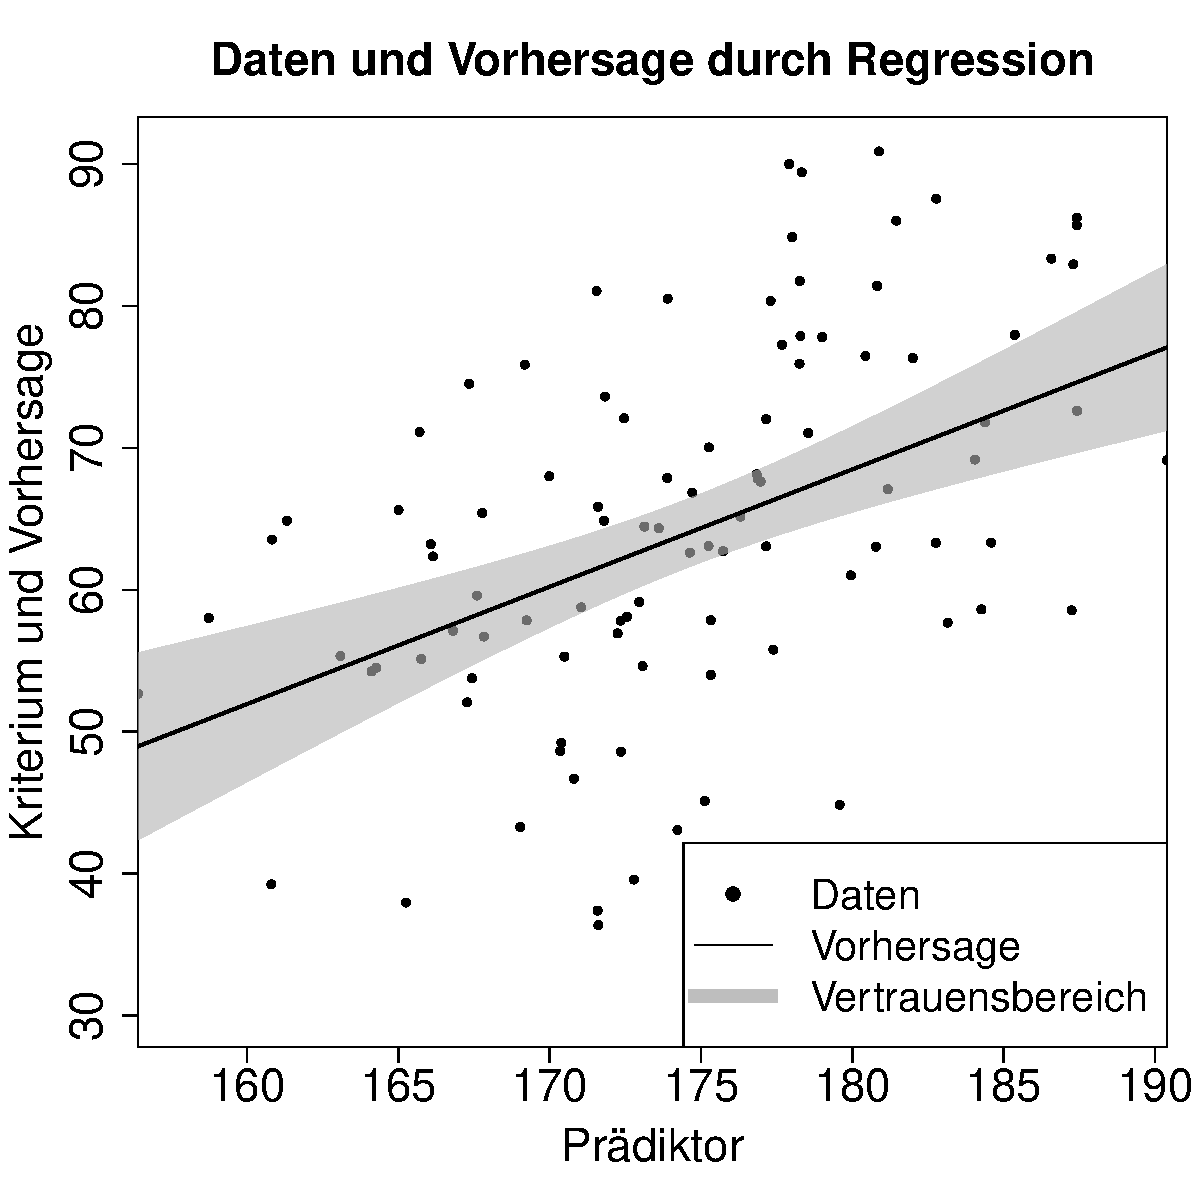
\includegraphics[width=8cm]{regrCI}
\vspace*{-1em}
\caption{Lineare Regression: Prädiktor, Kriterium und Vorhersage mit Vertrauensbereich}
\label{fig:regrCI}
\end{figure}

%%%%%%%%%%%%%%%%%%%%%%%%%%%%%%%%%%%%%%%%%%%%%%%%%%%%%%%%%%%%%%%%%%
%%%%%%%%%%%%%%%%%%%%%%%%%%%%%%%%%%%%%%%%%%%%%%%%%%%%%%%%%%%%%%%%%%
\section{Regressionsdiagnostik}
\label{sec:regrDiag}
%%%%%%%%%%%%%%%%%%%%%%%%%%%%%%%%%%%%%%%%%%%%%%%%%%%%%%%%%%%%%%%%%%
%%%%%%%%%%%%%%%%%%%%%%%%%%%%%%%%%%%%%%%%%%%%%%%%%%%%%%%%%%%%%%%%%%

\index{Regression!Regressionsdiagnostik}
\index{Regression!Voraussetzungen}
Einer konventionellen Regressionsanalyse liegen verschiedene Annahmen zugrunde, deren Gültigkeit vorauszusetzen ist, damit die berechneten Standardfehler der Parameterschätzungen und die $p$-Werte korrekt sind (Abschn.\ \ref{sec:multALMpred}). Dazu gehören Normalverteiltheit und gemeinsame Unabhängigkeit der Messfehler des Kriteriums, die zudem unabhängig von den Prädiktoren sein müssen. Hinzu kommt die \emph{Homoskedastizität}, also die Gleichheit aller bedingten Fehlervarianzen (Abb.\ \ref{fig:regrHomSc}).

Mit Hilfe der Regressionsdiagnostik soll zum einen geprüft werden, ob die Daten mit den gemachten Annahmen konsistent sind. Zum anderen kann die Parameterschätzung der konventionellen Regression durch wenige Ausreißer überproportional beeinflusst werden. Daher ist es von Interesse, diese zu identifizieren und den Einfluss einzelner Beobachtungen auf das Ergebnis zu bestimmen. Schließlich ist in der multiplen Regression das Ausmaß der Multikollinearität bedeutsam, also die wechselseitige lineare Abhängigkeit der Prädiktoren untereinander. Für eine ausführliche Darstellung vgl.\ \citeA{Fox2002} sowie das zugehörige Paket \lstinline!car!\index[pack]{car@\lstinline{car}} für Funktionen, mit denen sich eine Vielzahl diagnostischer Diagramme erstellen lassen.

%%%%%%%%%%%%%%%%%%%%%%%%%%%%%%%%%%%%%%%%%%%%%%%%%%%%%%%%%%%%%%%%%%
%%%%%%%%%%%%%%%%%%%%%%%%%%%%%%%%%%%%%%%%%%%%%%%%%%%%%%%%%%%%%%%%%%
\subsection{Extremwerte, Ausreißer und Einfluss}
\label{sec:regrInfluence}
%%%%%%%%%%%%%%%%%%%%%%%%%%%%%%%%%%%%%%%%%%%%%%%%%%%%%%%%%%%%%%%%%%
%%%%%%%%%%%%%%%%%%%%%%%%%%%%%%%%%%%%%%%%%%%%%%%%%%%%%%%%%%%%%%%%%%

\index{Daten!Ausreißer}
\index{Daten!Extremwerte}
Unter einem Ausreißer sind hier Beobachtungen zu verstehen, deren Kriteriumswert stark vom Kriteriumswert anderer Beobachtungen abweicht, die ähnliche Prädiktorwerte besitzen. Extremwerte einer gegebenen Variable zeichnen sich dadurch aus, dass sie weit außerhalb der Verteilung der übrigen Beobachtungen liegen. Die grafische Beurteilung, ob Extremwerte vorliegen, lässt sich getrennt für jede Variable etwa durch Histogramme oder boxplots der $z$-standardisierten Variable durchführen (Abb.\ \ref{fig:regrInfl}; Abschn.\ \ref{sec:hist}, \ref{sec:boxplot}).

Als numerische Indikatoren eignen sich die $z$-standardisierten Werte, an denen abzulesen ist, wie viele Streuungseinheiten ein Wert vom Mittelwert entfernt ist. Als numerisches Maß der multivariaten Extremwertanalyse bietet sich die Mahalanobisdistanz als Verallgemeinerung der $z$-Transformation an (Abschn.\ \ref{sec:mahaDist}). Sie repräsentiert den Abstand eines Datenpunkts zum Zentroid der Verteilung, wobei der Gesamtform der Verteilung i.\,S.\ der Kovarianzmatrix Rechnung getragen wird. Für die grafische Darstellung der gemeinsamen Verteilung von zwei oder drei Variablen s.\ Abschn.\ \ref{sec:distr2var}, \ref{sec:3dPlot}.\footnote{\index{robuste Verfahren!Ausreißer identifizieren}Da Extremwerte die Lage und Streuung der Daten mit beeinflussen, sollten hierfür evtl.\ robuste Schätzer in Betracht gezogen werden (Abschn.\ \ref{sec:varRob}). Robuste Schätzungen für die Kovarianzmatrix können etwa an das Argument \lstinline!cov! von \lstinline!mahalanobis()! übergeben werden. Für fortgeschrittene Tests, ob Ausreißer in multivariaten Daten vorliegen, vgl.\ \lstinline!aq.plot()!\index[func]{aq.plot()@\lstinline{aq.plot()}} und\index[func]{pcout()@\lstinline{pcout()}} \lstinline!pcout()! aus dem Paket \lstinline!mvoutlier!\index[pack]{mvoutlier@\lstinline{mvoutlier}} \cite{Filzmoser2011b}.}
\begin{lstlisting}
> Xpred <- cbind(height, age, sport)      # Prädiktoren als Datenmatrix
> Xz    <- scale(Xpred)                   # z-Transformierte
> boxplot(Xz, main="Verteilung standardisierte Prädiktoren")
> summary(Xz)
        height              age                 sport
Min.   :-2.534e+00  Min.   :-1.952e+00  Min.   :-1.796e+00
1st Qu.:-6.040e-01  1st Qu.:-7.110e-01  1st Qu.:-6.884e-01
Median : 1.075e-02  Median :-1.069e-01  Median :-9.467e-02
Mean   : 1.781e-15  Mean   :-8.978e-17  Mean   : 1.087e-16
3rd Qu.: 6.338e-01  3rd Qu.: 7.411e-01  3rd Qu.: 6.519e-01
Max.   : 2.200e+00  Max.   : 2.839e+00  Max.   : 2.727e+00

# Mahalanobis-Distanz der Beobachtungen zum Zentroid der Prädiktoren
> ctrX   <- colMeans(Xpred)               # Zentroid
> sX     <- cov(Xpred)                    # Kovarianzmatrix
> mahaSq <- mahalanobis(Xpred, ctrX, sX)  # quadrierte M-Distanzen
> summary(sqrt(mahaSq))
  Min.  1st Qu.  Median    Mean  3rd Qu.    Max.
0.2855   1.1640  1.5940  1.5970   1.9750  3.3090
\end{lstlisting}

\index{Regression!Hebelwert}
Durch Extremwerte oder Ausreißer wird die ermittelte Vorhersagegleichung womöglich in dem Sinne verzerrt, dass sie die Mehrzahl der Daten nicht mehr gut repräsentiert. Um den Einfluss der einzelnen Beobachtungen auf die Parameterschätzungen der Regression direkt zu quantifizieren, existieren verschiedene Kennwerte, darunter der Hebelwert $h$ (\emph{leverage}). $h$ wird durch\index[func]{hatvalues()@\lstinline{hatvalues()}} \lstinline!hatvalues(<<lm-Modell>>)! berechnet.\footnote{Zudem ist $h_{i}$ gleich dem $i$-ten Eintrag $\bm{H}_{ii}$ in der Diagonale der\index{Regression!Hat-Matrix} Hat-Matrix $\bm{H}$ (Abschn.\ \ref{sec:regrMultAn}).} Für Modelle, die einen absoluten Term $b_{0}$ einschließen, kann $h$ Werte im Intervall $[\frac{1}{n}, 1]$ annehmen, wobei $n$ die Anzahl an Beobachtungen ist. Der Mittelwert ist dann gleich $\frac{p+1}{n}$ mit $p+1$ als Anzahl zu schätzender Parameter der Regression ($p$ Prädiktoren sowie absoluter Term). Um besonders große Hebelwerte zu identifizieren, kann ihre Verteilung etwa über ein Histogramm oder einen \emph{spike-plot} veranschaulicht werden (Abb.\ \ref{fig:regrInfl}, Abschn.\ \ref{sec:plot}). Als numerisches Kriterium für auffällig große Hebelwerte dient bisweilen das Zwei- bis Dreifache seines Mittelwerts.
\begin{lstlisting}
> fitHAS <- lm(weight ~ height + age + sport)   # Regression
> h      <- hatvalues(fitHAS)                   # Hebelwerte
> hist(h, main="Histogramm der Hebelwerte")     # Histogramm
> summary(h)
   Min.  1st Qu.   Median     Mean  3rd Qu.     Max.
0.01082  0.02368  0.03568  0.04000  0.04942  0.12060
\end{lstlisting}

Zur Kontrolle lässt sich die Beziehung nutzen, dass die quadrierte Mahalanobisdistanz einer Beobachtung $i$ zum Zentroid der Prädiktoren gleich $(n-1) (h_{i} - \frac{1}{n})$ ist.
\begin{lstlisting}
> all.equal(mahaSq, (N-1) * (h - (1/N)), check.attributes=FALSE)
[1] TRUE
\end{lstlisting}

\index{Regression!Einfluss}
Die Indizes DfFITS bzw.\ DfBETAS liefern für jede Beobachtung ein standardisiertes Maß, wie stark sich die Vorhersagewerte (DfFITS) bzw.\ jeder geschätzte Parameter (DfBETAS) tatsächlich ändern, wenn die Beobachtung aus den Daten ausgeschlossen wird. In welchem Ausmaß sich dabei der Standardschätzfehler ändert, wird über das Verhältnis beider resultierenden Werte (mit bzw.\ ohne ausgeschlossene Beobachtung) ausgedrückt. Cooks Distanz ist ein weiteres Einflussmaß, das sich als $\frac{E^{2}}{\hat{\sigma}^{2} (1-h)^{2}} \cdot \frac{h}{p+1}$ berechnet, wobei $E$ für die Residuen $Y - \hat{Y}$ und $\hat{\sigma}$ für den Standardschätzfehler der Regression mit $p+1$ Parametern steht.

Mit\index[func]{influence.measures()@\lstinline{influence.measures()}} \lstinline!influence.measures(<<lm-Modell>>)! lassen sich die genannten Kennwerte gleichzeitig berechnen. Auffällige Beobachtungen können aus der zurückgegebenen Liste mit\index[func]{summary()@\lstinline{summary()}} \lstinline!summary()! extrahiert werden, wobei der Wert der abweichenden diagnostischen Größe durch einen Stern \lstinline!*! markiert ist.
\begin{lstlisting}
> inflRes <- influence.measures(fitHAS)    # Diagnosegrößen
> summary(inflRes)                         # auffällige Beobachtungen
Potentially influential observations of
lm(formula = weight ~ height + age + sport) :
    dfb.1  dfb.hght  dfb.age  dfb.sprt  dffit   cov.r    cook.d   hat
6   -0.05      0.07    -0.23      0.25   0.40    0.86_*    0.04  0.03
13  -0.21      0.21    -0.10      0.36   0.41    1.13_*    0.04  0.12_*
30   0.19     -0.23     0.17     -0.01  -0.42    0.74_*    0.04  0.02
31  -0.08      0.11    -0.08     -0.05   0.27    0.86_*    0.02  0.01
67   0.02     -0.02    -0.03      0.03  -0.05    1.17_*    0.00  0.11
72  -0.03      0.03     0.04      0.01   0.05    1.17_*    0.00  0.11
86   0.10     -0.16     0.60     -0.25   0.68_*  0.90      0.11  0.08
97  -0.01      0.01    -0.01      0.01   0.02    1.16_*    0.00  0.10
\end{lstlisting}

In der Ausgabe beziehen sich die Spalten \lstinline!dfb.<<Prädiktor>>! auf das DfBETA jedes Prädiktors (inkl.\ des absoluten Terms \lstinline!1! in der ersten Spalte), \lstinline!dffit! auf DfFITS, \lstinline!cov.r! auf das Verhältnis der Standardschätzfehler, \lstinline!cook.d! auf Cooks Distanz und \lstinline!hat! auf den Hebelwert. Für Funktionen zur separaten Berechnung der Maße vgl.\ \lstinline!?influence.measures!.
\begin{lstlisting}
> cooksDst <- cooks.distance(fitHAS)               # Cooks Distanz
> plot(cooksDst, main="Cooks Distanz", type="h")   # spike-plot

# manuelle Berechnung
> P   <- 3                                         # Anzahl Prädiktoren
> E   <- residuals(fitHAS)                         # Residuen
> MSE <- sum(E^2) / (N - (P+1))           # quadr. Standardschätzfehler
> CD  <- (E^2 / (MSE * (1-h)^2)) * (h / (P+1))     # Cooks Distanz
> all.equal(cooksDst, CD)                          # Kontrolle
[1] TRUE
\end{lstlisting}

Grafisch aufbereitete Informationen über den Einfluss einzelner Beobachtungen sowie über die Verteilung der Residuen (s.\,u.) liefert auch eine mit\index[func]{plot()@\lstinline{plot()}} \lstinline!plot(<<lm-Modell>>, which=1:6)! aufzurufende Serie von Diagrammen. Über das Argument \lstinline!which! können dabei einzelne Grafiken der Serie selektiv gezeigt werden. Vergleiche dazu auch\index[func]{influencePlot()@\lstinline{influencePlot()}} \lstinline!influencePlot()! und\index[func]{influenceIndexPlot()@\lstinline{influenceIndexPlot()}} \lstinline!influenceIndexPlot()! aus dem \index[pack]{car@\lstinline{car}} \lstinline!car! Paket.

\begin{figure}[ht]
\centering
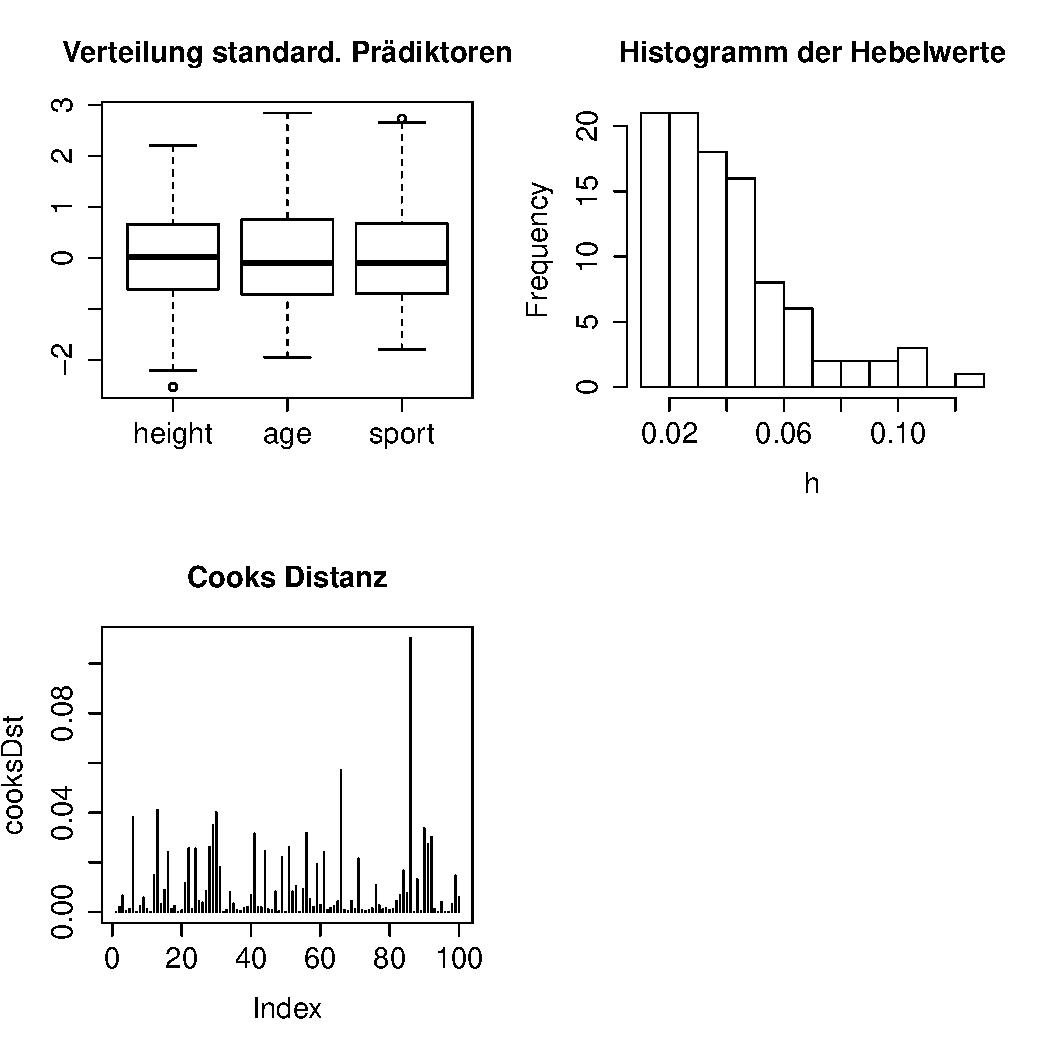
\includegraphics[width=12.5cm]{regrInfl}
\vspace*{-0.5em}
\caption{Beurteilung von Extremwerten und Einflussgrößen in der Regression}
\label{fig:regrInfl}
\end{figure}

%%%%%%%%%%%%%%%%%%%%%%%%%%%%%%%%%%%%%%%%%%%%%%%%%%%%%%%%%%%%%%%%%%
%%%%%%%%%%%%%%%%%%%%%%%%%%%%%%%%%%%%%%%%%%%%%%%%%%%%%%%%%%%%%%%%%%
\subsection{Verteilungseigenschaften der Residuen}
\label{sec:regrResid}
%%%%%%%%%%%%%%%%%%%%%%%%%%%%%%%%%%%%%%%%%%%%%%%%%%%%%%%%%%%%%%%%%%
%%%%%%%%%%%%%%%%%%%%%%%%%%%%%%%%%%%%%%%%%%%%%%%%%%%%%%%%%%%%%%%%%%

Die Verteilung der Residuen in Abhängigkeit von einzelnen Prädiktoren kann in einer multiplen Regression das Verständnis der Zusammenhänge erleichtern. Das Paket \lstinline!car!\index[pack]{car@\lstinline{car}} bietet hierfür die Funktion \index[func]{residualPlots()@\lstinline{residualPlots()}}\lstinline!residualPlots()! mit zahlreichen Optionen (Abb.\ \ref{fig:regrResidPlot}).

\begin{lstlisting}
> library(car)                    # für residualPlots()
> residualPlots(fitHAS, tests=FALSE)
\end{lstlisting}

\begin{figure}[ht]
\centering
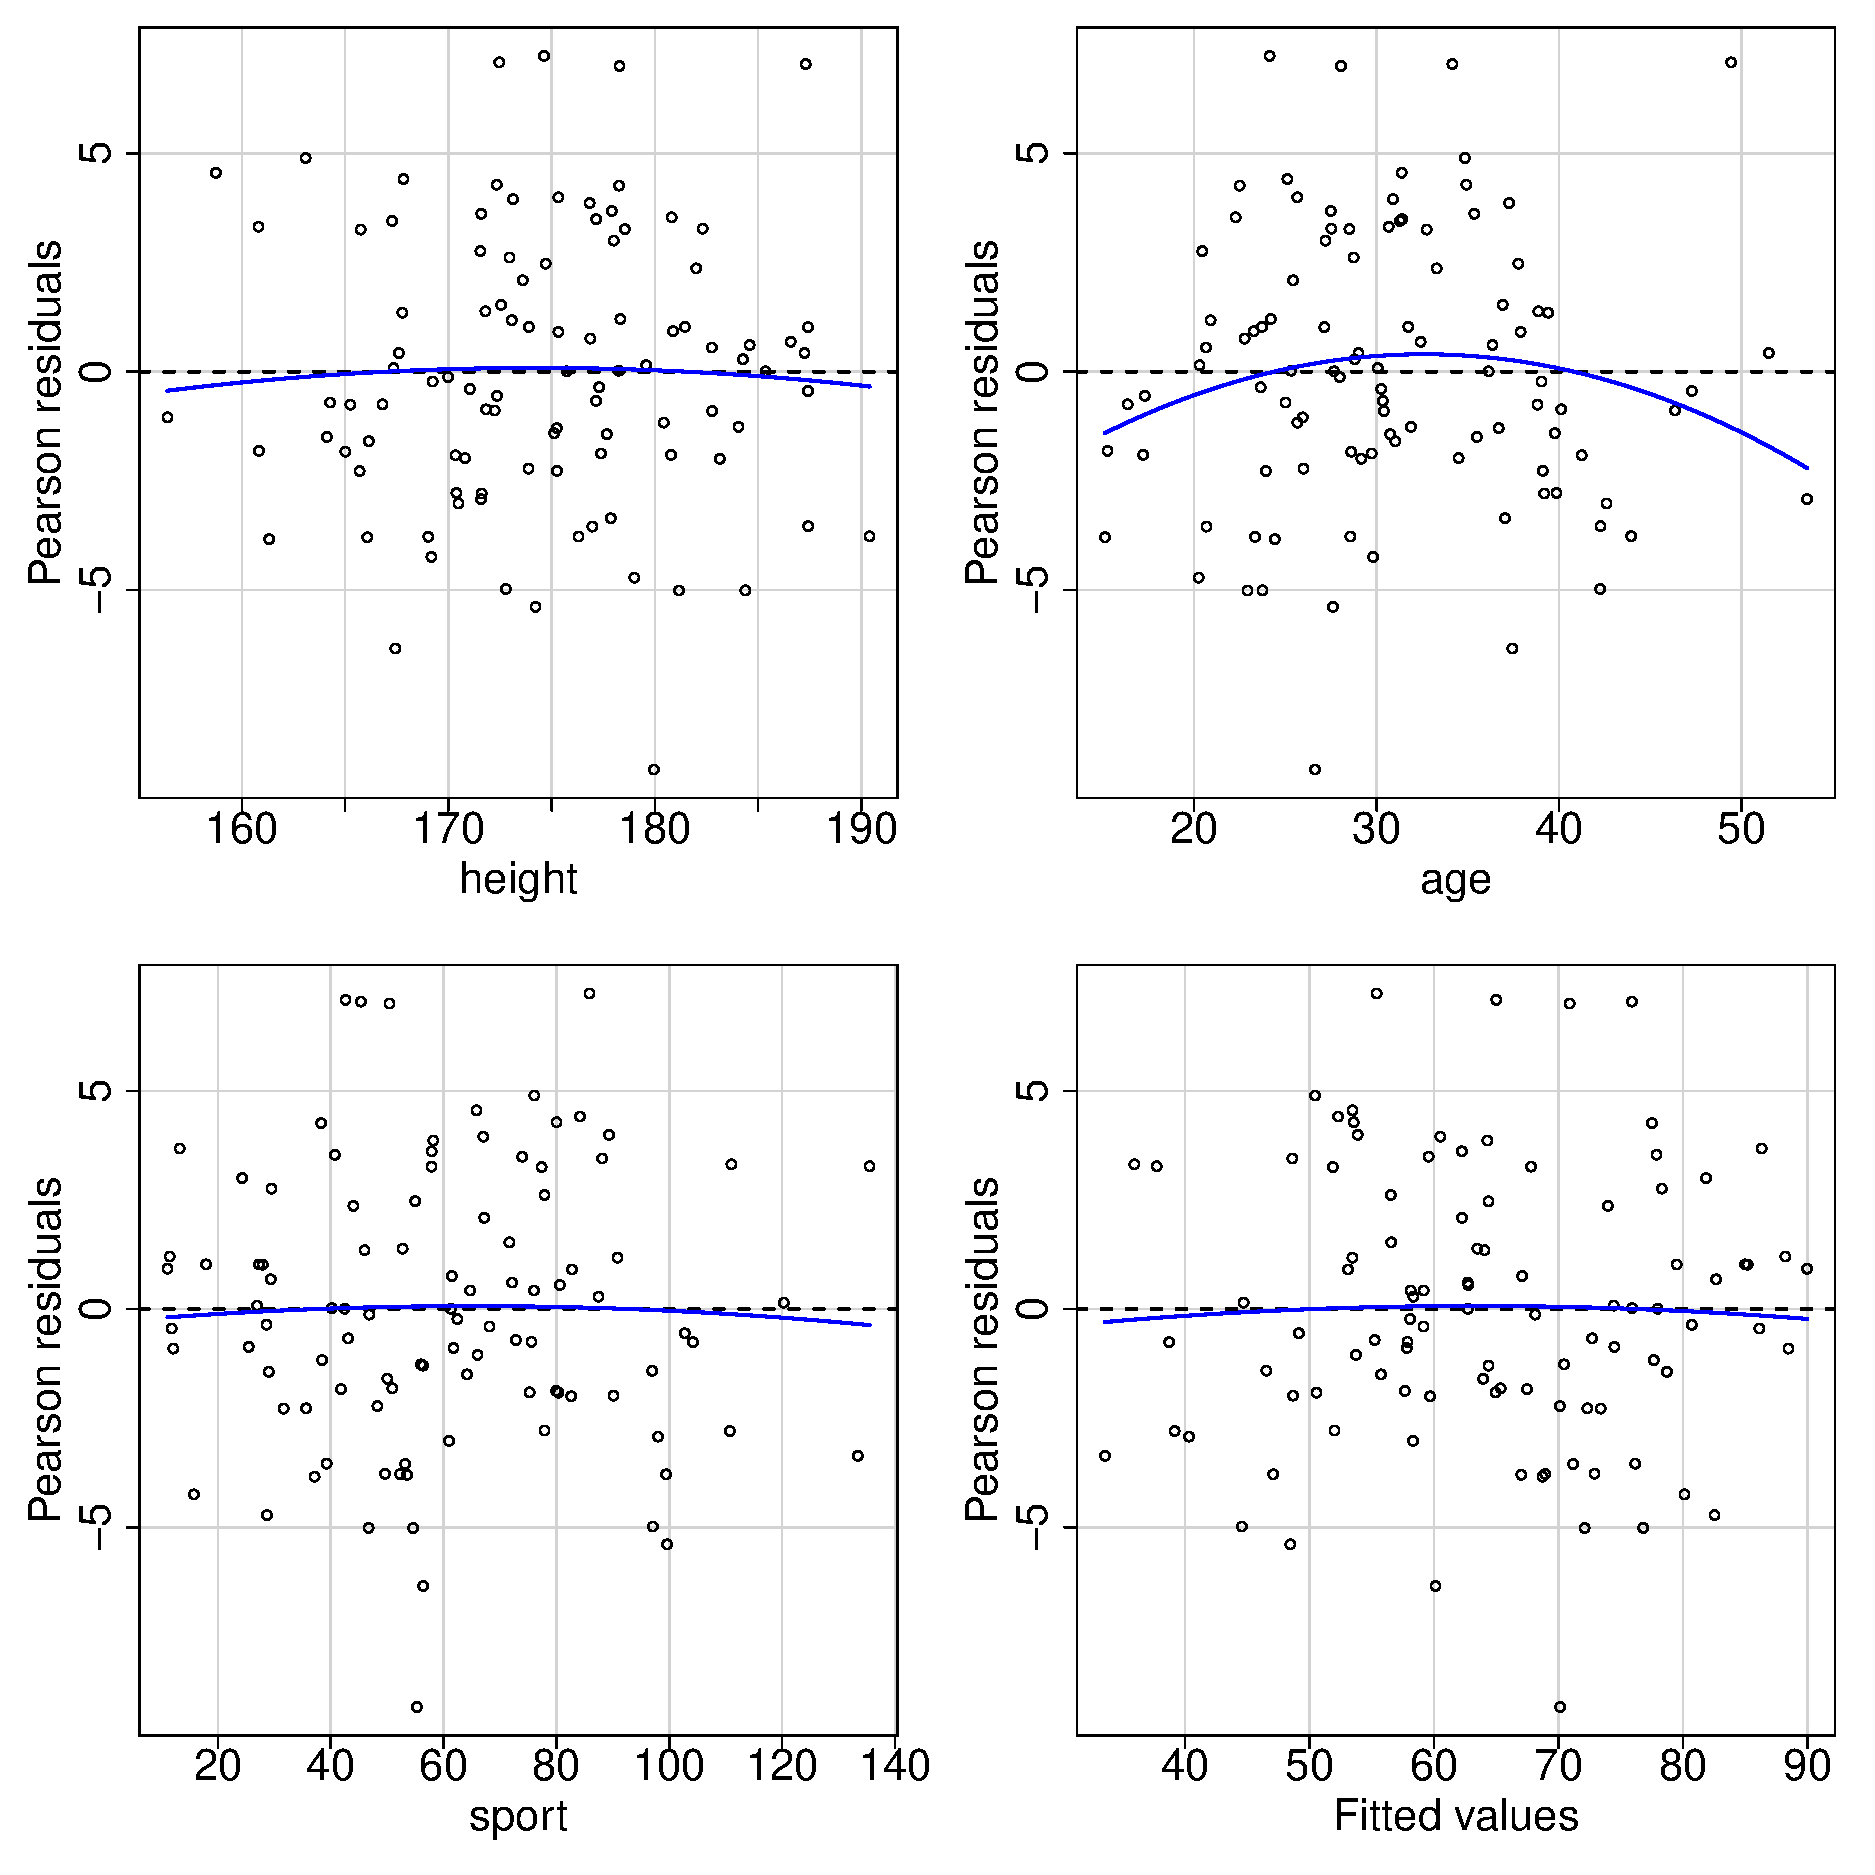
\includegraphics[width=12.5cm]{regrResidPlot}
\vspace*{-0.5em}
\caption{Prädiktor-Residuen Diagramme in der multiple Regression}
\label{fig:regrResidPlot}
\end{figure}

Anhand verschiedener grafischer Darstellungen der Residuen einer Regression lässt sich heuristisch beurteilen, ob die vorliegenden Daten mit den Voraussetzungen der Normalverteiltheit, Unabhängigkeit und Homoskedastizität der Messfehler vereinbar sind. Als Grundlage können die Residuen $E = Y - \hat{Y}$ selbst, oder aber zwei Transformationen von ihnen dienen: Die \emph{standardisierten} und \emph{studentisierten} Residuen besitzen eine theoretische Streuung von $1$ und ergeben sich als $\frac{E}{\hat{\sigma} \sqrt{1-h}}$, wobei $\hat{\sigma}$ eine Schätzung der theoretischen Fehlerstreuung ist (Abschn.\ \ref{sec:multALMpred}).

Für die standardisierten Residuen wird der Standardschätzfehler als globale Schätzung in der Rolle von $\hat{\sigma}$ verwendet, bei den studentisierten Residuen dagegen eine beobachtungsweise Schätzung $\hat{\sigma}_{i}$. Dabei wird im Fall \emph{extern} studentisierter Residuen (\emph{leave-one-out}) $\hat{\sigma}_{(i)}$ für jede Beobachtung $i$ auf Basis des Regressionsmodells berechnet, in das alle Daten bis auf die der $i$-ten Beobachtung einfließen. Für die im Folgenden aufgeführten Prüfmöglichkeiten werden oft standardisierte oder studentisierte Residuen $E$ gegenüber vorgezogen.

\lstinline!lm.influence()!\index[func]{lm.influence()@\lstinline{lm.influence()}} speichert $\hat{\sigma}_{(i)}$ in der Komponente \lstinline!sigma! der ausgegebenen Liste. Die Residuen selbst lassen sich mit \lstinline!residuals()! für $E$, \lstinline!rstandard()!\index[func]{rstandard()@\lstinline{rstandard()}} für die standardisierten und\index[func]{rstudent()@\lstinline{rstudent()}} \lstinline!rstudent()! für die extern studentisierten Residuen ermitteln (s.\ auch Abschn.\ \ref{sec:LOOCV}). Bei allen Funktionen ist als Argument ein von \lstinline!lm()! erstelltes Modell zu übergeben.
\begin{lstlisting}
> Estnd <- rstandard(fitHAS)                # standardisierte Residuen
> all.equal(Estnd, E / sqrt(MSE * (1-h)))   # manuelle Kontrolle
[1] TRUE

# studentisierte Residuen und manuelle Kontrolle
> Estud <- rstudent(fitHAS)
> all.equal(Estud, E / (lm.influence(fitHAS)$sigma * sqrt(1-h)))
[1] TRUE
\end{lstlisting}

Für eine visuell-exploratorische Beurteilung der Normalverteiltheit wird die Verteilung der bevorzugten Residuen-Variante mit einem Histogramm der relativen Klassenhäufigkeiten dargestellt, dem die Dichtefunktion der Standardnormalverteilung hinzugefügt wurde (Abb.\ \ref{fig:regrResid}, Abschn.\ \ref{sec:hist}). Das Histogramm sollte in seiner Form nicht stark von der Dichtefunktion abweichen. Zudem lässt sich ein Q-Q-plot nutzen, um die empirischen Quantile der Residuen mit jenen der Standardnormalverteilung zu vergleichen. Die Datenpunkte sollten hier auf einer Geraden liegen (Abb.\ \ref{fig:regrResid}, Abschn.\ \ref{sec:qq}). Für einen inferenzstatistischen Test mit der $\text{H}_{0}$, dass Normalverteilung vorliegt, bietet sich jener nach Shapiro-Wilk an.
\begin{lstlisting}
> hist(Estud, main="Histogramm studentisierte Residuen", freq=FALSE)

# Dichtefunktion der Standardnormalverteilung hinzufügen
> curve(dnorm(x, mean=0, sd=1), col="red", lwd=2, add=TRUE)
> qqnorm(Estud, main="Q-Q-Plot studentisierte Residuen")     # Q-Q-plot
> qqline(Estud, col="red", lwd=2) # Referenzgerade für Normalverteilung

# Shapiro-Wilk-Test auf Normalverteilung der studentisierten Residuen
> shapiro.test(Estud)
Shapiro-Wilk normality test
data: Estud
W = 0.9879, p-value = 0.4978
\end{lstlisting}

\index{Regression!Homoskedastizität}
Soll eingeschätzt werden, ob die Annahme von Homoskedastizität plausibel ist, kann die bevorzugte Residuen-Variante auf der Ordinate gegen die Vorhersage auf der Abszisse abgetragen werden (\emph{spread-level-plot}, Abb.\ \ref{fig:regrResid}).\footnote{Mitunter werden hierfür auch die Beträge der Residuen bzw.\ deren Wurzel gewählt (\emph{scale-location plot}). Der Breusch-Pagan-Test auf Heteroskedastizität kann mit\index[func]{bptest()@\lstinline{bptest()}} \lstinline!bptest()! aus dem Paket\index[pack]{lmtest@\lstinline{lmtest}|textbf} \lstinline!lmtest! \cite{Zeileis2002} durchgeführt werden.} Die Datenpunkte sollten überall gleichmäßig um die $0$-Linie streuen. Anhand desselben Diagramms kann auch die Unabhängigkeit der Messfehler heuristisch geprüft werden: Die Residuen sollten eine Verteilung aufweisen, die nicht systematisch mit der Vorhersage zusammenhängt.\footnote{Für den Durbin-Watson-Test auf Autokorrelation der Residuen vgl.\ \lstinline!durbinWatsonTest()!\index[func]{durbinWatsonTest()@\lstinline{durbinWatsonTest()}} aus dem Paket\index[pack]{car@\lstinline{car}} \lstinline!car!. Das Autokorrelations-Diagramm der Residuen erzeugt\index[func]{acf()@\lstinline{acf()}} \lstinline!acf(residuals(<<lm-Objekt>>))!.}
\begin{lstlisting}
# studentisierte Residuen gegen Vorhersage darstellen
> plot(fitted(fitHAS), Estud, pch=20, xlab="Vorhersage",
+      ylab="studentisierte Residuen", main="Spread-Level-Plot")

> abline(h=0, col="red", lwd=2)         # Referenz für Modellgültigkeit
\end{lstlisting}

\begin{figure}[ht]
\centering
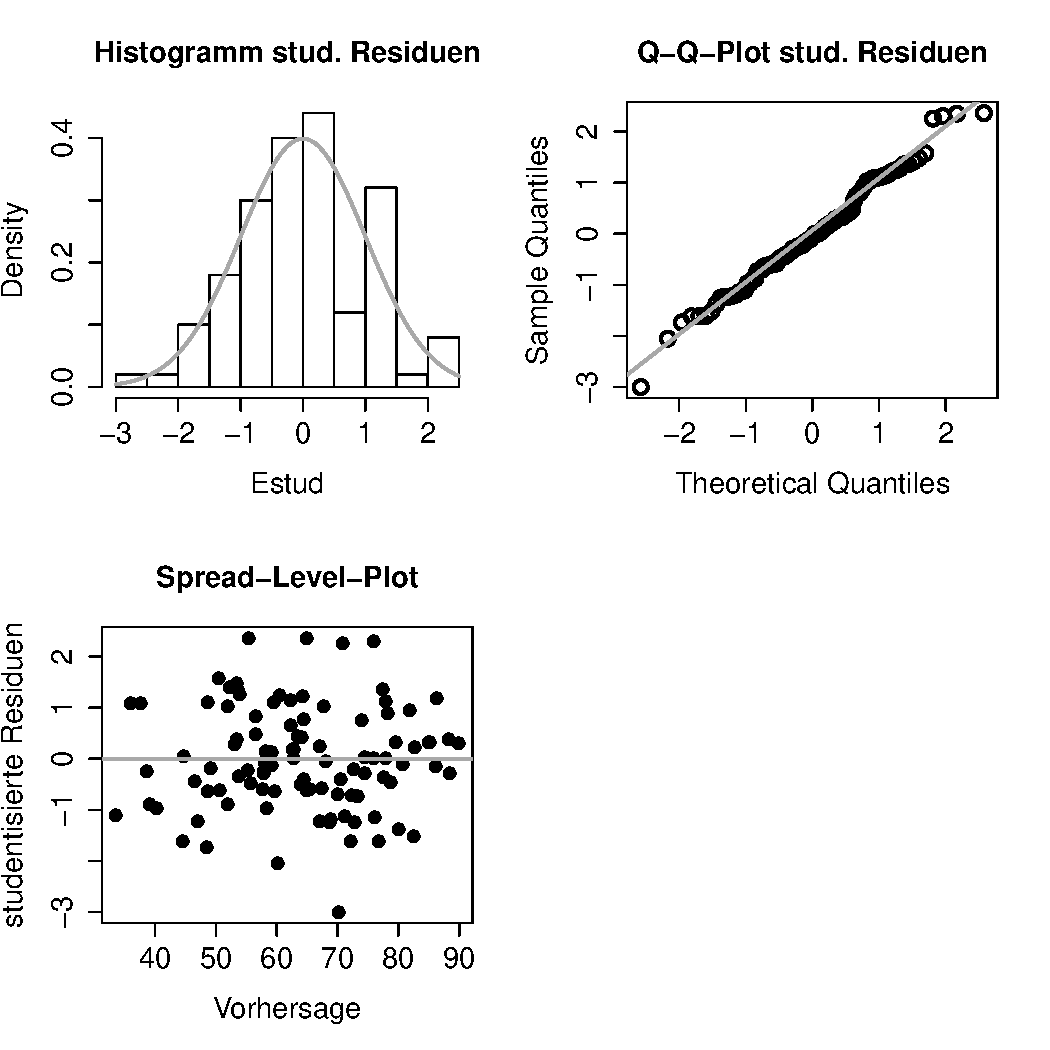
\includegraphics[width=12.5cm]{regrResid}
\vspace*{-0.5em}
\caption{Grafische Prüfung der Verteilungsvoraussetzungen für eine Regressionsanalyse}
\label{fig:regrResid}
\end{figure}

\index{Regression!Box-Cox-Transformation}
\index{Box-Cox-Transformation|see{Regression}}
Für manche Fälle, in denen die Daten darauf hindeuten, dass die Verteilung einer Variable $Y$ nicht den Voraussetzungen genügt, können streng monotone Transformationen die Verteilung günstig beeinflussen, bei echt positiven Daten etwa Potenzfunktionen der Form $Y^{\lambda}$: Dazu zählen der Kehrwert $Y^{-1}$, der Logarithmus $\ln Y$ (per definitionem für $\lambda = 0$), die Quadratwurzel $Y^{\frac{1}{2}}$ (z.\,B.\ bei absoluten Häufigkeiten), oder der Arkussinus der Quadratwurzel $\arcsin Y^{\frac{1}{2}}$ (z.\,B.\ bei Anteilen). In der Regression finden bisweilen Box-Cox-Transformationen $\frac{Y^{\lambda}-1}{\lambda}$ für $\lambda \neq 0$ bzw.\ $\ln Y$ für $\lambda = 0$ Verwendung, die ebenfalls echt positive Daten voraussetzen. Für sie stellt das Paket \lstinline!car!\index[pack]{car@\lstinline{car}} die in Kombination miteinander zu verwendenden Funktionen \index[func]{powerTransform()@\lstinline{powerTransform()}} \lstinline!powerTransform()! und \lstinline!bcPower()!\index[func]{bcPower()@\lstinline{bcPower()}} bereit.
\begin{lstlisting}
> powerTransform(<<lm-Modell>>, family="bcPower")
> bcPower(<<Vektor>>, <<lambda>>)
\end{lstlisting}

Als erstes Argument von \lstinline!powerTransform()! kann ein mit \lstinline!lm()! erstelltes Modell angegeben werden. Für die Maximum-Likelihood-Schätzung des Parameters $\lambda$ ist das Argument \lstinline!family! auf \lstinline!"bcPower"! zu setzen. $\lambda$ erhält man aus dem zurückgegebenen Objekt durch\index[func]{coef()@\lstinline{coef()}} \lstinline!coef()!. Die Box-Cox-Transformation selbst führt \lstinline!bcPower()! durch und benötigt dafür als Argument zum einen den Vektor der zu transformierenden Werte, zum anderen den Parameter $\lambda$ der Transformation.
\begin{lstlisting}
> library(car)                        # für boxCox(), powerTransform()
> lamObj  <- powerTransform(fitHAS, family="bcPower")
> (lambda <- coef(lamObj))            # max log-likelihood lambda
      Y1
1.057033

# transformiertes Kriterium und manuelle Kontrolle
> wTrans <- bcPower(weight, coef(lambda))       # Transformation
> all.equal(wTrans, ((weight^lambda) - 1) / lambda)   # manuell
[1] TRUE
\end{lstlisting}

%%%%%%%%%%%%%%%%%%%%%%%%%%%%%%%%%%%%%%%%%%%%%%%%%%%%%%%%%%%%%%%%%%
%%%%%%%%%%%%%%%%%%%%%%%%%%%%%%%%%%%%%%%%%%%%%%%%%%%%%%%%%%%%%%%%%%
\subsection{Multikollinearität}
\label{sec:multColl}
%%%%%%%%%%%%%%%%%%%%%%%%%%%%%%%%%%%%%%%%%%%%%%%%%%%%%%%%%%%%%%%%%%
%%%%%%%%%%%%%%%%%%%%%%%%%%%%%%%%%%%%%%%%%%%%%%%%%%%%%%%%%%%%%%%%%%

\index{Regression!Multikollinearität}
Multikollinearität liegt in einer multiplen Regression dann vor, wenn sich die Werte eines Prädiktors gut aus einer Linearkombination der übrigen Prädiktoren vorhersagen lassen. Dies ist insbesondere dann der Fall, wenn Prädiktoren paarweise miteinander korrelieren. Für die multiple Regression hat dies als unerwünschte Konsequenz einerseits weniger stabile Schätzungen der Koeffizienten zur Folge, die mit hohen Schätzfehlern versehen sind. Ebenso kann sich die Parameterschätzung bzgl.\ desselben Prädiktors stark in Abhängigkeit davon ändern, welche anderen Prädiktoren noch berücksichtigt werden. Andererseits ergeben sich Schwierigkeiten bei der Interpretation der $b_{j}$- bzw.\ der standardisierten $b_{j}^{z}$-Gewichte: Verglichen mit der Korrelation der zugehörigen Variable mit dem Kriterium können letztere unerwartet große oder kleine Werte annehmen und auch im Vorzeichen von der Korrelation abweichen.\footnote{Auf numerischer Seite bringt starke Multikollinearität das Problem mit sich, dass die interne Berechnung der Parameterschätzungen anfälliger für Fehler werden kann, die aus der notwendigen Ungenauigkeit der Repräsentation von Gleitkommazahlen in Computern herrühren (Abschn.\ \ref{sec:isTRUE}).}

Ob paarweise lineare Abhängigkeiten vorliegen, lässt sich anhand der Korrelationsmatrix $\bm{R}_{x}$ der Prädiktoren prüfen.
\begin{lstlisting}
> (Rx <- cor(cbind(height, age, sport)))      # Korrelationsmatrix
            height         age        sport
height  1.00000000  0.06782798  -0.20937559
age     0.06782798  1.00000000   0.09496699
sport  -0.20937559  0.09496699   1.00000000
\end{lstlisting}

\index{Regression!Varianzinflationsfaktor}
Die Diagonalelemente der Inversen $\bm{R}_{x}^{-1}$ liefern den \emph{Varianzinflationsfaktor} $\text{VIF}_{j}$ jedes Prädiktors $j$ als weitere Möglichkeit zur Kollinearitätsdiagnostik: $\sqrt{\text{VIF}_{j}}$ ist der Faktor, um den das Konfidenzintervall für das wahre $\beta_{j}$-Gewicht breiter als im analogen Fall linear unabhängiger Prädiktoren ist. $\text{VIF}_{j}$ berechnet sich alternativ als $\frac{1}{1-R_{j}^{2}}$, also als Kehrwert der Toleranz $1-R_{j}^{2}$, wobei $R_{j}^{2}$ der Determinationskoeffizient bei der Regression des Prädiktors $j$ auf alle übrigen Prädiktoren ist. Aus dem Paket\index[pack]{car@\lstinline{car}} \lstinline!car! stammt die Funktion \lstinline!vif(<<lm-Modell>>)!\index[func]{vif()@\lstinline{vif()}}, die als Argument ein durch \lstinline!lm()! erstelltes lineares Modell erwartet.
\begin{lstlisting}
> library(car)                                # für vif()
> vif(fitHAS)
  height       age     sport
1.054409  1.017361  1.059110
\end{lstlisting}

In der Ausgabe findet sich unter dem Namen jedes Prädiktors der zugehörige $\text{VIF}_{j}$-Wert. Da geringe Werte für die Toleranz auf lineare Abhängigkeit zwischen den Prädiktoren hindeuten, gilt dasselbe für große $\text{VIF}$-Werte. Konventionell werden $\text{VIF}$-Werte von bis zu ca.\ $4$ als unkritisch, jene über $10$ als starke Indikatoren für Multikollinearität gewertet. Es folgt die manuelle Kontrolle anhand der Regressionen jeweils eines Prädiktors auf alle übrigen.
\begin{lstlisting}
# Regression jeweils eines Prädiktors auf alle übrigen
> fitHeight <- lm(height ~ age    + sport)
> fitAge    <- lm(age    ~ height + sport)
> fitSport  <- lm(sport  ~ height + age)

# VIF_j aus zugehörigem Determinationskoeffizienten R^2
> 1 / (1 - summary(fitHeight)$r.squared)      # VIF height
[1] 1.054409

> 1 / (1 - summary(fitAge)$r.squared)         # VIF age
[1] 1.017361

> 1 / (1 - summary(fitSport)$r.squared)       # VIF sport
[1] 1.05911

# alternativ: Diagonalelemente der Inversen der Korrelationsmatrix
> diag(solve(Rx))
  height       age     sport
1.054409  1.017361  1.059110
\end{lstlisting}

Ein weiterer Kennwert zur Beurteilung von Multikollinearität ist die\index{Matrix!Kondition $\kappa$} Kondition $\kappa$ der Designmatrix $\bm{X}$ des meist mit standardisierten Variablen gebildeten linearen Modells (Abschn.\ \ref{sec:matProp}, \ref{sec:multALMregr}). Werte von $\kappa > 20$ sprechen einer Faustregel folgend für Multikollinearität. Zur Berechnung dient\index[func]{kappa()@\lstinline{kappa()}} \lstinline!kappa(<<lm-Modell>>, exact=FALSE)!, wobei für eine numerisch aufwendigere, aber präzisere Bestimmung von $\kappa$ das Argument \lstinline!exact=TRUE! zu setzen ist. Neben $\kappa$ eignen sich zur differenzierteren Diagnose auch die Eigenwerte von $\bm{X}^{\top} \bm{X}$ selbst sowie ihr jeweiliger Konditionsindex.\footnote{Fortgeschrittene Methoden zur Diagnostik von Multikollinearität enthält das Paket \lstinline!perturb!\index[pack]{perturb@\lstinline{perturb}} \cite{Hendrickx2008}.}
\begin{lstlisting}
# Regressionsmodell mit standardisierten Prädiktoren
> lmScl <- lm(scale(weight) ~ scale(height) + scale(age) + scale(sport))
> kappa(lmScl, exact=TRUE)
[1] 1.279833

> X        <- model.matrix(lmScl)             # Designmatrix
> (eigVals <- eigen(t(X) %*% X)$values)       # Eigenwerte von X^t * X
[1] 119.93081 103.85018 100.00000  73.21902

# Konditionsindizes: jeweils Wurzel aus Eigenwert / (Minimum != 0)
> sqrt(eigVals / min(eigVals[eigVals >= .Machine$double.eps]))
[1] 1.279833 1.190945 1.168660 1.000000
\end{lstlisting}

Wenn von den ursprünglichen Variablen zu zentrierten oder standardisierten Variablen übergangen wird, ändern sich die $\text{VIF}_{j}$ Werte nur dann, wenn multiplikative Terme, also Interaktionen in der Regression einbezogen sind (Abschn.\ \ref{sec:regrMod}). Dagegen ändert sich $\kappa$ bei solchen Variablentransformationen praktisch immer.\footnote{Ursache dafür ist die Änderung der Eigenwerte bei Datentransformationen: Ist $\bm{X}$ die Designmatrix des ursprünglichen Modells und $\bm{X}'$ die Designmatrix des Modells der transformierten Daten, so gehen die Eigenwerte von $(\bm{X}')^{\top} \bm{X}'$ nicht auf einfache Weise aus denen von $\bm{X}^{\top} \bm{X}$ hervor. Insbesondere verändern sich der größte und kleinste Eigenwert jeweils unterschiedlich, so dass deren Quotient nicht konstant ist.}
\begin{lstlisting}
# VIF: Regression mit standardisierten Variablen -> kein Unterschied
> vif(lmScl)
scale(height)  scale(age)  scale(sport)
     1.054409    1.017361      1.059110

# kappa: Regression mit ursprünglichen Variablen -> Unterschied
> kappa(lm(weight ~ height + age + sport), exact=TRUE)
[1] 4804.947
\end{lstlisting}

%%%%%%%%%%%%%%%%%%%%%%%%%%%%%%%%%%%%%%%%%%%%%%%%%%%%%%%%%%%%%%%%%%
%%%%%%%%%%%%%%%%%%%%%%%%%%%%%%%%%%%%%%%%%%%%%%%%%%%%%%%%%%%%%%%%%%
%\newpage
\section{Erweiterungen der linearen Regression}
\label{sec:lmExtend}
%%%%%%%%%%%%%%%%%%%%%%%%%%%%%%%%%%%%%%%%%%%%%%%%%%%%%%%%%%%%%%%%%%
%%%%%%%%%%%%%%%%%%%%%%%%%%%%%%%%%%%%%%%%%%%%%%%%%%%%%%%%%%%%%%%%%%

%%%%%%%%%%%%%%%%%%%%%%%%%%%%%%%%%%%%%%%%%%%%%%%%%%%%%%%%%%%%%%%%%%
%%%%%%%%%%%%%%%%%%%%%%%%%%%%%%%%%%%%%%%%%%%%%%%%%%%%%%%%%%%%%%%%%%
\subsection{Robuste Regression}
\label{sec:lmRob}
%%%%%%%%%%%%%%%%%%%%%%%%%%%%%%%%%%%%%%%%%%%%%%%%%%%%%%%%%%%%%%%%%%
%%%%%%%%%%%%%%%%%%%%%%%%%%%%%%%%%%%%%%%%%%%%%%%%%%%%%%%%%%%%%%%%%%

\index{Regression!robuste}
\index{robuste Verfahren!Regression}
Die Parameterschätzung \emph{robuster} Regressionsverfahren soll weniger sensibel auf die Verletzung von Voraussetzungen und auf die Anwesenheit von Ausreißern reagieren. Das Paket \lstinline!robustbase!\index[pack]{robustbase@\lstinline{robustbase}} stellt für zwei Varianten der robusten Regression\index[func]{lmrob()@\lstinline{lmrob()}} \lstinline!lmrob()! und \index[func]{ltsReg()@\lstinline{ltsReg()}} \lstinline!ltsReg()! bereit. Einen Überblick über weitere Quellen gibt der Abschnitt \emph{Robust Statistical Methods} der CRAN Task Views \cite{CRANtvRobust}.
\begin{lstlisting}
> library(robustbase)                       # für lmrob()
> fitLMR <- lmrob(weight ~ height + age + sport, setting="KS2014")
> summary(fitLMR)                           # gekürzte Ausgabe ...
Residuals:
    Min      1Q  Median      3Q     Max 
-9.1512 -1.9595 -0.1204  2.4366  7.2985 

Coefficients:
            Estimate Std. Error t value Pr(>|t|)    
(Intercept)  7.97897    8.41419   0.948    0.345    
height       0.51710    0.04732  10.927  < 2e-16 ***
age         -0.29663    0.04175  -7.105 2.11e-10 ***
sport       -0.41546    0.01230 -33.785  < 2e-16 ***

Robust residual standard error: 3.21 
Multiple R-squared:  0.9458,    Adjusted R-squared:  0.9441
\end{lstlisting}

Allgemein können Bootstrap-Verfahren geeignet sein, trotz verletzter Modellvoraussetzungen angemessene Standardfehler der Parameterschätzungen zu erhalten (Abschn.\ \ref{sec:bootRegr}).

Speziell für Schätzungen der Standardfehler der Regression unter Heteroskedastizität vgl.\ \lstinline!sandwich(<<lm-Modell>>)!\index[func]{sandwich()@\lstinline{sandwich()}} und \lstinline!vcovHC(<<lm-Modell>>)!\index[func]{vcovHC()@\lstinline{vcovHC()}} aus dem Paket\index[pack]{sandwich@\lstinline{sandwich}|textbf} \lstinline!sandwich! \cite{Zeileis2004}. Diese Funktionen bestimmen die Kovarianzmatrix der Parameterschätzer eines mit \lstinline!lm()! angepassten Modells neu. Wald-Tests der Parameter können dann mit\index[func]{coeftest()@\lstinline{coeftest()}} \lstinline!coeftest(<<lm-Modell>>, vcov=<<Schätzer>>)! aus dem Paket \index[pack]{lmtest@\lstinline{lmtest}} \lstinline!lmtest! durchgeführt werden, wobei für das Argument \lstinline!vcov! das Ergebnis von \lstinline!sandwich()! oder \lstinline!vcovHC()! anzugeben ist.
\begin{lstlisting}
> library(sandwich)                       # für vcovHC()
> library(lmtest)                         # für coeftest()
> hcSE <- vcovHC(fitHAS, type="HC3")
> coeftest(fitHAS, vcov=hcSE)
t test of coefficients:

             Estimate Std. Error  t value  Pr(>|t|)
(Intercept)  8.101233   8.083794   1.0022    0.3188
height       0.514893   0.046507  11.0714 < 2.2e-16 ***
age         -0.286646   0.042196  -6.7932 9.177e-10 ***
sport       -0.415952   0.011293 -36.8330 < 2.2e-16 ***
\end{lstlisting}

%%%%%%%%%%%%%%%%%%%%%%%%%%%%%%%%%%%%%%%%%%%%%%%%%%%%%%%%%%%%%%%%%%
%%%%%%%%%%%%%%%%%%%%%%%%%%%%%%%%%%%%%%%%%%%%%%%%%%%%%%%%%%%%%%%%%%
\subsection{Penalisierte Regression}
\label{sec:lmPen}
%%%%%%%%%%%%%%%%%%%%%%%%%%%%%%%%%%%%%%%%%%%%%%%%%%%%%%%%%%%%%%%%%%
%%%%%%%%%%%%%%%%%%%%%%%%%%%%%%%%%%%%%%%%%%%%%%%%%%%%%%%%%%%%%%%%%%

\index{Regression!penalisierte}
Bei hoher Multikollinearität und in Situationen mit sehr vielen Prädiktoren (relativ zur Anzahl verfügbarer Beobachtungen), kommen \emph{penalisierte} Regressionsverfahren in Betracht. Sie beschränken den geschätzten Parametervektor $\hat{\bm{\beta}}$ ohne $\hat{\beta_{0}}$ in seiner Norm, reduzieren also den Betrag der Parameterschätzungen (\emph{shrinkage}). Die resultierenden Parameterschätzungen sind nicht mehr unverzerrt, für den Preis eines geringen bias können sie jedoch eine deutlich geringere Varianz der Schätzungen aufweisen als die übliche lineare Regression. Penalisierte Regressionen werden üblicherweise mit standardisierten Prädiktoren und Kriterium durchgeführt.

\index{Regression!Ridge-Regression}
Die Ridge-Regression wird durch \lstinline!lm.ridge()!\index[func]{lm.ridge()@\lstinline{lm.ridge()}} aus dem\index[pack]{MASS@\lstinline{MASS}|textbf} \lstinline!MASS! Paket \cite{Venables2002} bereitgestellt. Die Funktion akzeptiert eine Modellformel und für das Argument \lstinline!lambda! den Wert des Tuning-Parameters $\lambda$. Dieser kontrolliert, wie stark das shrinkage ausfällt. Im ersten Schritt empfiehlt es sich, für \lstinline!lambda! einen Vektor mit vielen Werten zu übergeben, etwa im Intervall $[0.01, 10000]$. \lstinline!lm.ridge()! berechnet dann für jeden Wert von $\lambda$ den Vorhersagefehler aus der verallgemeinerten Kreuzvalidierung (GCV, s.\ Abschn.\ \ref{sec:LOOCV} sowie Abb.\ \ref{fig:penalized}).
\begin{lstlisting}
> library(MASS)                             # für lm.ridge(), select()
> lambdas  <- 10^(seq(-2, 4, length=100))   # Tuning-Parameter
> ridgeGCV <- lm.ridge(scale(weight) ~ scale(height) + scale(age) +
+                                      scale(sport), lambda=lambdas)
\end{lstlisting}

Im Anschluss erfährt man mit\index[func]{select()@\lstinline{select()}} \lstinline!select(<<lm.ridge-Objekt>>)!, für welchen Wert von $\lambda$ der Kreuzvalidierungsfehler sein Minimum erreicht.
\begin{lstlisting}
> select(ridgeGCV)
modified HKB estimator is 0.06879525
modified L-W estimator is 0.06014114
smallest value of GCV  at 0.2477076
\end{lstlisting}

In einem erneuten Aufruf von \lstinline!lm.ridge()! kann schließlich \lstinline!lambda! auf den vorher identifizierten Wert mit dem geringsten Kreuzvalidierungsfehler gesetzt werden. Aus dem erzeugten Objekt extrahiert \lstinline!coef()! dann die Parameterschätzungen.
\begin{lstlisting}
# lambda für geringsten Kreuzvalidierungsfehler
> lambda   <- ridgeGCV$lambda[ridgeGCV$GCV == min(ridgeGCV$GCV)]
> ridgeSel <- lm.ridge(scale(weight) ~ scale(height) + scale(age) +
+                                      scale(sport), lambda=lambda)

> coef(ridgeSel)                            # Parameterschätzungen
               scale(height)     scale(age)   scale(sport)
-3.765673e-16   2.743740e-01  -1.706931e-01  -8.475898e-01
\end{lstlisting}

\index{Regression!LASSO}
\index{Regression!elastic net}
Die Methoden LASSO und elastic net wählen anders als die Ridge-Regression gleichzeitig auch eine Teilmenge von Prädiktoren aus, indem sie abhängig von $\lambda$ einzelne Parameterschätzungen auf $0$ reduzieren. Eine Umsetzung von ridge, LASSO und elastic net liefern \lstinline!cv.glmnet()!\index[func]{cv.glmnet()@\lstinline{cv.glmnet()}} sowie \lstinline!glmnet()!\index[func]{glmnet()@\lstinline{glmnet()}} aus dem Paket\index[pack]{glmnet@\lstinline{glmnet}|textbf} \lstinline!glmnet! \cite{Friedman2010}.

Anders als die bisher vorgestellten Funktionen akzeptieren \lstinline!cv.glmnet()! und \lstinline!glmnet()! keine Modellformel.\footnote{Das Paket\index[pack]{glmnetUtils@\lstinline{glmnetUtils}} \lstinline!glmnetUtils! \cite{Ooi2017} bietet aber eine entsprechende Erweiterung an.} Stattdessen muss für \lstinline!x! die Matrix der Prädiktoren übergeben werden und für \lstinline!y! der Vektor der modellierten Zielvariable. Dabei berechnet die Funktion \lstinline!cv.glmnet()! für von ihr selbst gewählte Werte von $\lambda$ den Vorhersagefehler aus der verallgemeinerten Kreuzvalidierung für \lstinline!nfolds! viele Partitionen (Abschn.\ \ref{sec:LOOCV}). Die zurückgegebene Liste speichert in der Komponente \lstinline!lambda.min! den Wert für $\lambda$, der den Kreuzvalidierungsfehler minimiert. Für die Ridge-Regression ist das Argument \lstinline!alpha=0! zu setzen. Der Regularisierungspfad -- hier der Verlauf der Parameterschätzungen $\hat{\beta}_{j}$ in Abhängigkeit von $\ln \lambda$ -- ist in Abb.\ \ref{fig:penalized} dargestellt.
\begin{lstlisting}
# Matrix der standardisierten Prädiktoren und des Kriteriums
> matScl <- scale(cbind(weight, height, age, sport))
> library(glmnet)                           # für cv.glmnet(), glmnet()

# verallgemeinerte Kreuzvalidierung für lambda - Ridge-Regression
> ridgeCV <- cv.glmnet(matScl[ , c("height", "age", "sport")],
+                      matScl[ , "weight"], nfolds=10, alpha=0)
\end{lstlisting}

Anschließend passt \lstinline!glmnet()! das Modell für einen konkreten Wert von $\lambda$ an und gibt ein Objekt zurück, aus dem sich mit \lstinline!coef()! die Parameterschätzungen extrahieren lassen.
\begin{lstlisting}
> ridge <- glmnet(matScl[ , c("height", "age", "sport")],
+                 matScl[ , "weight"],
+                 lambda=ridgeCV$lambda.min, alpha=0)

> coef(ridge)                               # Parameterschätzungen
(Intercept) -3.837235e-16
height       2.640929e-01
age         -1.618367e-01
sport       -7.806060e-01

# oder direkt ohne Anpassung mit glmnet()
> coef(ridgeCV, s=ridgeCV$lambda.min)       # ...
\end{lstlisting}

Für das LASSO-Verfahren ist in \lstinline!cv.glmnet()! und \lstinline!glmnet()! das Argument \lstinline!alpha=1! zu setzen. Der Regularisierungspfad -- hier der Verlauf der Parameterschätzungen in Abhängigkeit von der $L_{1}$-Norm $\sum_{j} |\hat{\beta}_{j}|$ des Vektors $\hat{\bm{\beta}}$ -- ist in Abb.\ \ref{fig:penalized} dargestellt.
\begin{lstlisting}
# verallgemeinerte Kreuzvalidierung für lambda - LASSO
> lassoCV <- cv.glmnet(matScl[ , c("height", "age", "sport")],
+                      matScl[ , "weight"], nfolds=10, alpha=1)

> lasso <- glmnet(matScl[ , c("height", "age", "sport")],
+                 matScl[ , "weight"],
+                 lambda=lassoCV$lambda.min, alpha=1)

> coef(lasso)                               # Parameterschätzungen
(Intercept) -3.886238e-16
height       2.708041e-01
age         -1.667786e-01
sport       -8.466213e-01

# oder direkt ohne Anpassung mit glmnet()
> coef(lassoCV, s=lassoCV$lambda.min)       # ...
\end{lstlisting}

Für das elastic-net-Verfahren ist in \lstinline!cv.glmnet()! und \lstinline!glmnet()! das Argument \lstinline!alpha=0.5! zu setzen. Der Regularisierungspfad -- hier der Verlauf der Parameterschätzungen $\hat{\beta}_{j}$ in Abhängigkeit vom Anteil der aufgeklärten Devianz -- ist in Abb.\ \ref{fig:penalized} dargestellt.
\begin{lstlisting}
# verallgemeinerte Kreuzvalidierung für lambda - elastic net
> elNetCV <- cv.glmnet(matScl[ , c("height", "age", "sport")],
+                      matScl[ , "weight"], nfolds=10, alpha=0.5)

> elNet <- glmnet(matScl[ , c("height", "age", "sport")],
+                 matScl[ , "weight"],
+                 lambda=elNetCV$lambda.min, alpha=0.5)

> coef(elNet)                               # Parameterschätzungen
(Intercept) -3.899363e-16
height       2.713961e-01
age         -1.674823e-01
sport       -8.447744e-01

# oder direkt ohne Anpassung mit glmnet()
> coef(elNetCV, s=elNetCV$lambda.min)       # ...
\end{lstlisting}

\begin{figure}[ht]
\centering
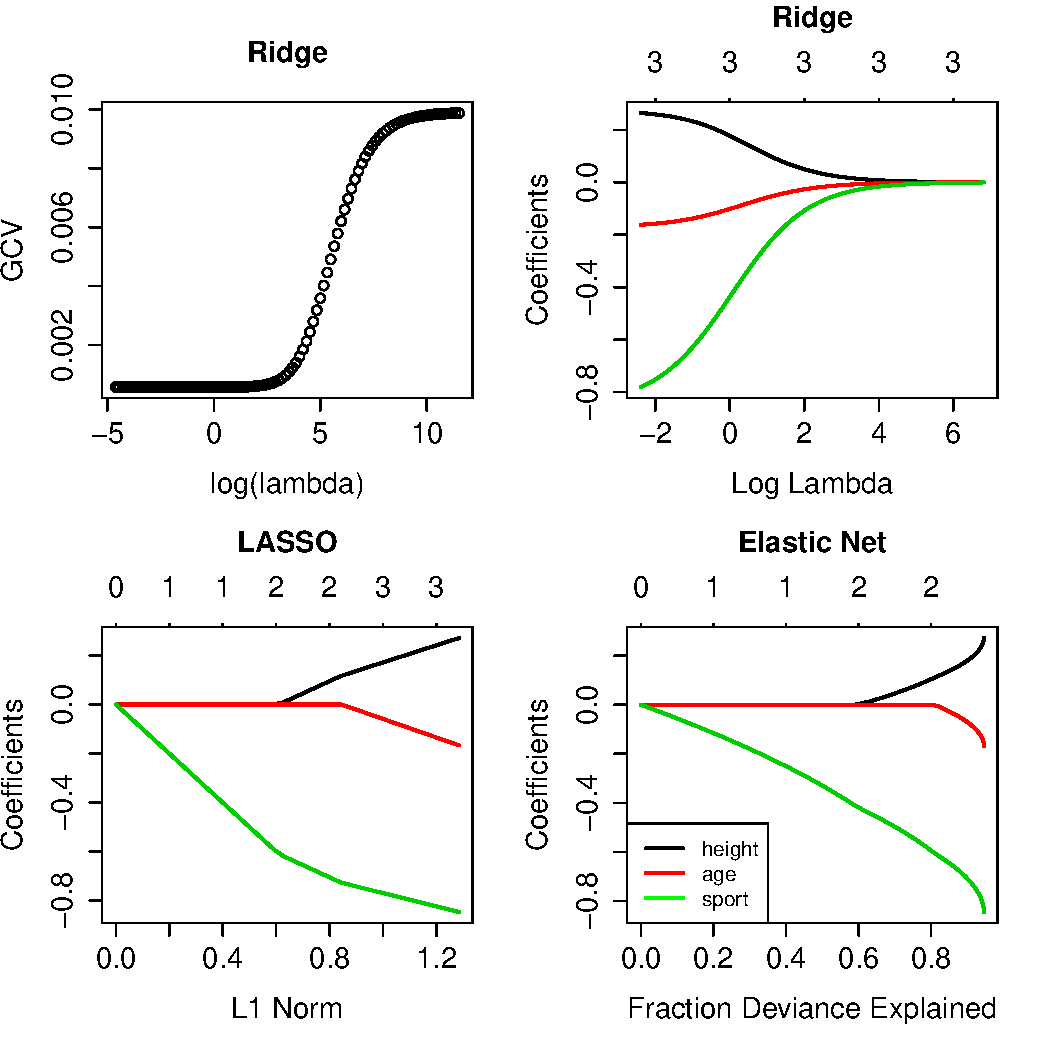
\includegraphics[width=12.5cm]{penalized}
\vspace*{-0.5em}
\caption{Penalisierte Regression: Kreuzvalidierungsfehler in Abhängigkeit von $\ln \lambda$ in der Ridge-Regression mit \lstinline!lm.ridge()!. Regularisierungspfade für Ridge-Regression, LASSO und elastic net mit \lstinline!glmnet()!. Die obere $x$-Achse zeigt die Anzahl ausgewählter Parameter $\hat{\beta}_{j} \neq 0$.}
\label{fig:penalized}
\end{figure}

%%%%%%%%%%%%%%%%%%%%%%%%%%%%%%%%%%%%%%%%%%%%%%%%%%%%%%%%%%%%%%%%%%
%%%%%%%%%%%%%%%%%%%%%%%%%%%%%%%%%%%%%%%%%%%%%%%%%%%%%%%%%%%%%%%%%%
\subsection{Nichtlineare Zusammenhänge}
\label{sec:lmNonlin}
%%%%%%%%%%%%%%%%%%%%%%%%%%%%%%%%%%%%%%%%%%%%%%%%%%%%%%%%%%%%%%%%%%
%%%%%%%%%%%%%%%%%%%%%%%%%%%%%%%%%%%%%%%%%%%%%%%%%%%%%%%%%%%%%%%%%%

Ein Regressionsmodell, das linear in den Parametern ist, kann dennoch das Kriterium als nichtlineare Funktion einzelner Prädiktoren beschreiben. So erleichtert es die Funktion\index{Regression!polynomiale} \lstinline!poly(<<Prädiktor>>, degree=<<Grad>>)!\index[func]{poly()@\lstinline{poly()}}, orthogonale Polynome für eine polynomiale Regression mit quadratischen Termen oder Polynomen höheren Grades zu erstellen. Analog stellt das im Basisumfang von R enthaltene Paket\index[pack]{splines@\lstinline{splines}} \lstinline!splines! mit \lstinline!ns(<<Prädiktor>>, df=<<Grad>>)!\index[func]{ns()@\lstinline{ns()}} natürliche\index{splines} splines (außerhalb des beobachteten Wertebereichs linear) und mit \lstinline!bs(<<Prädiktor>>, df=<<Grad>>)!\index[func]{bs()@\lstinline{bs()}} $B$-splines (mit Bernstein-Polynomen als Basis-Funktionen) zur Verfügung. Beide Funktionen können innerhalb der Modellformel von \lstinline!lm()! verwendet werden und besitzen das Argument \lstinline!df!, um ihre Variabilität zu kontrollieren.

Verallgemeinerte additive Modelle werden durch die Funktion\index[func]{gam()@\lstinline{gam()}} \lstinline!gam()! aus dem Paket\index[pack]{mgcv@\lstinline{mgcv}} \lstinline!mgcv! \cite{Wood2006} unterstützt. Sie kann automatisch die Variabilitätsparameter einer Vielzahl von Spline-Typen auswählen und lässt auch Interaktionen von Spline-Termen mit anderen Kovariaten zu.

Für die Bestimmung von Parametern in nichtlinearen Vorhersagemodellen\index{Regression!nichtlineare} anhand der Methode der kleinsten quadrierten Abweichungen vgl.\ \lstinline!nls()!\index[func]{nls()@\lstinline{nls()}} sowie \citeA{Ritz2009}.

%%%%%%%%%%%%%%%%%%%%%%%%%%%%%%%%%%%%%%%%%%%%%%%%%%%%%%%%%%%%%%%%%%
%%%%%%%%%%%%%%%%%%%%%%%%%%%%%%%%%%%%%%%%%%%%%%%%%%%%%%%%%%%%%%%%%%
\subsection{Abhängige Fehler bei Messwiederholung oder Clusterung}
\label{sec:lmLongitudinal}
%%%%%%%%%%%%%%%%%%%%%%%%%%%%%%%%%%%%%%%%%%%%%%%%%%%%%%%%%%%%%%%%%%
%%%%%%%%%%%%%%%%%%%%%%%%%%%%%%%%%%%%%%%%%%%%%%%%%%%%%%%%%%%%%%%%%%

Liefert eine Person mehrere Beobachtungen zu unterschiedlichen Zeitpunkten, sind die einzelnen Messwerte nicht mehr unabhängig voneinander. Dies ist auch der Fall, wenn verschiedene Personen aufgrund eines gemeinsamen Merkmals cluster bilden, z.\,B.\ durch eine familiäre Verwandtschaft. Eine wesentliche Voraussetzung der linearen Regressionsanalyse ist dann verletzt. Sowohl gemischte Modelle (\emph{linear mixed effects models}) als auch verallgemeinerte Schätzgleichungen (\emph{generalized estimating equations}, GEE) kommen für abhängige Daten in Betracht. Beide Herangehensweisen sind auch für kategoriale Zielvariablen in verallgemeinerten linearen Modellen wie der logistischen Regression oder der Poisson-Regression anwendbar (Kap.\ \ref{sec:glm}).

\index{gemischte Modelle}
Gemischte Modelle \cite{Pinheiro2000, West2006} können Abhängigkeitsstrukturen von Daten flexibel berücksichtigen. Sie werden von den Paketen \lstinline!lme4!\index[pack]{lme4@\lstinline{lme4}} \cite{Bates2008} sowie \lstinline!nlme!\index[pack]{nlme@\lstinline{nlme}} \cite{Pinheiro2008} unterstützt und eignen sich auch für Situationen, in denen nicht alle Personen dieselbe Anzahl von Messwerten zu denselben Zeitpunkten liefern. Die Abstände zwischen Zeitpunkten können variieren. Gemischte Modelle können kategoriale und kontinuierliche Prädiktoren einbeziehen, die auch zeitabhängig, d.\,h.\ innerhalb einer Person veränderlich sein dürfen. In varianzanalytischen Designs mit Messwiederholung (Abschn.\ \ref{sec:RBp}, \ref{sec:RBFpq}, \ref{sec:SPFpq}) bieten gemischte Modelle häufig eine alternative Möglichkeit zur Auswertung, die die Abhängigkeitsstruktur der Messungen besser als die klassische Varianzanalyse berücksichtigen kann.

\index{GEE (generalized estimating equations)}
\index{Verallgemeinerte Schätzgleichungen}
Verallgemeinerte Schätzgleichungen (GEE) modellieren die Abhängigkeit des bedingten Erwartungswerts der Zielvariable von den Prädiktoren getrennt von der Abhängigkeitsstruktur der Daten derselben Person oder desselben clusters. GEE sind im Paket \lstinline!geepack!\index[pack]{geepack@\lstinline{geepack}} \cite{Hojsgaard2006,Yan2004} implementiert.

%%%%%%%%%%%%%%%%%%%%%%%%%%%%%%%%%%%%%%%%%%%%%%%%%%%%%%%%%%%%%%%%%%
%%%%%%%%%%%%%%%%%%%%%%%%%%%%%%%%%%%%%%%%%%%%%%%%%%%%%%%%%%%%%%%%%%
\subsection{Regressionsmodelle für mehrere Verteilungsparameter}
\label{sec:gamlss}
%%%%%%%%%%%%%%%%%%%%%%%%%%%%%%%%%%%%%%%%%%%%%%%%%%%%%%%%%%%%%%%%%%
%%%%%%%%%%%%%%%%%%%%%%%%%%%%%%%%%%%%%%%%%%%%%%%%%%%%%%%%%%%%%%%%%%

In der einfachen linearen Regression wird nur der Erwartungswert als Lageparameter der bedingten Verteilung der vorhergesagten Variable als Linearkombination der Kovariaten modelliert. Mit Funktionen aus dem Paket \lstinline!gamlss!\index[pack]{gamlss@\lstinline{gamlss}} \cite{Stasinopoulos2017} ist es möglich, gleichzeitig auch ein Modell für die Streuung als zusätzlichen Parameter der bedingten Verteilung anzupassen und als Funktion von Kovariaten zu schätzen. Dies ist in verallgemeinerten linearen Modellen (Kap.\ \ref{sec:glm}) auch für bedingte Verteilungen möglich, die keine Normalverteilung sind und auch noch über einen ebenfalls modellierbaren Formparameter verfügen können.

%%%%%%%%%%%%%%%%%%%%%%%%%%%%%%%%%%%%%%%%%%%%%%%%%%%%%%%%%%%%%%%%%%
%%%%%%%%%%%%%%%%%%%%%%%%%%%%%%%%%%%%%%%%%%%%%%%%%%%%%%%%%%%%%%%%%%
\section{Partialkorrelation und Semipartialkorrelation}
\label{sec:partCorReg}
%%%%%%%%%%%%%%%%%%%%%%%%%%%%%%%%%%%%%%%%%%%%%%%%%%%%%%%%%%%%%%%%%%
%%%%%%%%%%%%%%%%%%%%%%%%%%%%%%%%%%%%%%%%%%%%%%%%%%%%%%%%%%%%%%%%%%

\index{Korrelation!Partialkorrelation}
Ein von \lstinline!lm()! erzeugtes Objekt kann auch zur Ermittlung der Partialkorrelation $r_{(XY).Z}$ zweier Variablen $X$ und $Y$ ohne eine dritte Variable $Z$ verwendet werden (Abschn.\ \ref{sec:covCor}): $r_{(XY).Z}$ ist gleich der Korrelation der Residuen der Regressionen jeweils von $X$ und $Y$ auf $Z$.
\begin{lstlisting}
# Partialkorrelation weight mit height, beide ohne sport
> weight.S <- residuals(lm(weight ~ sport)) # Resid.: weight ohne sport
> height.S <- residuals(lm(height ~ sport)) # Resid.: height ohne sport
> cor(weight.S, height.S)
[1] 0.6595016
\end{lstlisting}

Zur Kontrolle lässt sich die konventionelle Formel umsetzen oder der Umstand nutzen, dass Partialkorrelationen aus der invertierten Korrelationsmatrix $\bm{R}^{-1}$ der drei beteiligten Variablen berechnet werden können: Ist $\bm{D}$ die Diagonalmatrix aus den Diagonalelementen von $\bm{R}^{-1}$, stehen die Partialkorrelationen außerhalb der Diagonale der Matrix $-(\bm{D}^{-\frac{1}{2}} \bm{R}^{-1} \bm{D}^{-\frac{1}{2}})$ (s.\ Abschn.\ \ref{sec:linAlg} für Multiplikation und Invertierung von Matrizen).
\begin{lstlisting}
# Kontrolle über herkömmliche Formel
> (cor(weight, height) - (cor(weight, sport) * cor(height, sport))) /
+      sqrt((1-cor(weight, sport)^2) * (1-cor(height, sport)^2))
[1] 0.6595016

# Kontrolle über Inverse der Korrelationsmatrix
> R        <- cor(cbind(weight, height, sport))    # Korrelationsmatrix
> Rinv     <- solve(R)                      # ihre Inverse R^(-1)
> DsqrtInv <- diag(1/sqrt(diag(Rinv)))      # D^(-1/2)
> Rpart    <- -(DsqrtInv %*% Rinv %*% DsqrtInv)
> Rpart[upper.tri(Rpart)]                   # alle Partialkorrelationen
[1] 0.6595016 -0.9468826 0.5738578
\end{lstlisting}

Gleichzeitig beinhaltet $-(\bm{D}^{-1} \bm{R}^{-1})$ außerhalb der Diagonale die standardisierten $b_{j}^{z}$-Gewichte der Regressionen mit jeweils dem durch die Zeile definierten Kriterium und den durch die Spalten definierten Prädiktoren.
\begin{lstlisting}
> Dinv <- diag(1/diag(Rinv))                # D^(-1)
> bz   <- -(Dinv %*% Rinv)                  # -(D^(-1) * R^(-1))
> bz[upper.tri(bz)]                         # alle bz-Gewichte
[1] 0.2589668 -0.8691255  1.3414126

# standardisierte Regression weight auf height und sport
> fit <- lm(scale(weight) ~ scale(height) + scale(sport))
> zapsmall(coef(fit))                       # bz-Gewichte
(Intercept)  scale(height)  scale(sport)
  0.0000000      0.2589668    -0.8691255
\end{lstlisting}

\index{Korrelation!Semipartialkorrelation}
Die Semipartialkorrelation $r_{(X.Z)Y} = \frac{r_{XY} - (r_{XZ} \cdot r_{YZ})}{\sqrt{1-r_{XZ}^{2}}}$ einer Variable $Y$ mit einer Variable $X$ ohne $Z$ lässt sich analog zur Partialkorrelation als Korrelation von $Y$ mit den Residuen der Regression von $X$ auf $Z$ berechnen.
\begin{lstlisting}
# Semipartialkorrelation weight mit height ohne sport
> cor(weight, height.S)
[1] 0.2532269

# Kontrolle über herkömmliche Formel
> (cor(weight, height) - (cor(weight, sport) * cor(height, sport))) /
+      sqrt(1-cor(height, sport)^2)
[1] 0.2532269
\end{lstlisting}

Partialkorrelation und Semipartialkorrelation lassen sich auf die Situation verallgemeinern, dass nicht nur eine Variable $Z$ auspartialisiert wird, sondern mehrere Variablen $Z_{j}$. Die Partialkorrelation $r_{(XY).Z_{j}}$ ist dann die Korrelation der Residuen der multiplen Regression von $X$ auf alle $Z_{j}$ mit den Residuen der multiplen Regression von $Y$ auf alle $Z_{j}$. Ebenso ist die Semipartialkorrelation $r_{(X.Z_{j})Y}$ die Korrelation von $Y$ mit den Residuen der multiplen Regression von $X$ auf alle $Z_{j}$.
\begin{lstlisting}
# Residuen Regression von weight bzw. height auf verbleibende Variablen
> weight.AS <- residuals(lm(weight ~ age + sport))
> height.AS <- residuals(lm(height ~ age + sport))

# Partialkorrelation (weight mit height) ohne verbleibende Variablen
> (pcorWH.AS  <- cor(weight.AS, height.AS))
[1] 0.7531376

# Semipartialkorrelation weight mit (height ohne restliche Variablen)
> (spcorWH.AS <- cor(weight, height.AS))
[1] 0.2674680
\end{lstlisting}

Die Semipartialkorrelation $r_{(X.Z_{j})Y}$ weist folgenden Zusammenhang zur multiplen Regression des Kriteriums $Y$ auf die Prädiktoren $X$ und $Z_{j}$ auf: $r_{(X.Z_{j})Y}^{2}$ ist gleich der Erhöhung des Determinationskoeffizienten $R^{2}$ beim Übergang von der Regression von $Y$ auf $Z_{j}$ hin zur Regression von $Y$ auf die Prädiktoren $X$ und $Z_{j}$. In diesem Sinne ist die quadrierte Semipartialkorrelation des Kriteriums mit einem Prädiktor ohne alle übrigen gleich dem Varianzanteil, den der Prädiktor zusätzlich zu allen übrigen Prädiktoren aufklärt.
\begin{lstlisting}
> spcorWH.AS^2                  # quadrierte Semipartialkorrelation
[1] 0.07153911

# R^2 Differenz: Regressionen mit vs. ohne height inkl. übrige Prädikt.
> fitAS  <- lm(weight ~ age + sport)              # ohne height
> fitHAS <- lm(weight ~ height + age + sport)     # mit height
> summary(fitHAS)$r.squared - summary(fitAS)$r.squared
[1] 0.07153911
\end{lstlisting}

Ist $b_{x}$ das Regressionsgewicht des Prädiktors $X$ in der Regression des Kriteriums $Y$ auf die Prädiktoren $X$ und $Z_{j}$, und ist weiterhin $X.Z_{j}$ die Variable der Residuen der Regression von $X$ auf alle $Z_{j}$, so gilt analog zur einfachen linearen Regression $b_{x} = \frac{K_{(X.Z_{j})Y}}{s^{2}_{X.Z_{j}}}$, wenn $K$ für die Kovarianz und $s^{2}$ für die Varianz von Variablen steht.
\begin{lstlisting}
> fitHAS                    # multiple Regression, gekürzte Ausgabe ...
Coefficients:
(Intercept)  height      age    sport
     8.1012  0.5149  -0.2866  -0.4160

# b-Gewicht von height
> cov(weight, height.AS) / var(height.AS)
[1] 0.5148935
\end{lstlisting}
